\documentclass[review]{elsarticle}

\usepackage{xcolor}
\usepackage{
  , coqdoc
}[color]

\usepackage{lineno,hyperref}
\modulolinenumbers[5]
\usepackage{graphicx,hyperref}
\usepackage{float}
\usepackage{proof,tikz,minted}
\usepackage{amssymb,amsthm,stmaryrd}


\usetikzlibrary{automata}
\usetikzlibrary{shapes}
\usetikzlibrary{backgrounds}
\usetikzlibrary{positioning}
\usetikzlibrary{arrows}


\journal{Science of Computer Programming}

%%%%%%%%%%%%%%%%%%%%%%%
%% Elsevier bibliography styles
%%%%%%%%%%%%%%%%%%%%%%%
%% To change the style, put a % in front of the second line of the current style and
%% remove the % from the second line of the style you would like to use.
%%%%%%%%%%%%%%%%%%%%%%%

%% Numbered
%\bibliographystyle{model1-num-names}

%% Numbered without titles
%\bibliographystyle{model1a-num-names}

%% Harvard
%\bibliographystyle{model2-names.bst}\biboptions{authoryear}

%% Vancouver numbered
%\usepackage{numcompress}\bibliographystyle{model3-num-names}

%% Vancouver name/year
%\usepackage{numcompress}\bibliographystyle{model4-names}\biboptions{authoryear}

%% APA style
%\bibliographystyle{model5-names}\biboptions{authoryear}

%% AMA style
%\usepackage{numcompress}\bibliographystyle{model6-num-names}

%% `Elsevier LaTeX' style
\bibliographystyle{elsarticle-num}
%%%%%%%%%%%%%%%%%%%%%%%

\newcommand{\Eps}{\textit{Eps}}
\newcommand{\Chr}{\textit{Chr}}
\newcommand{\Catt}{\textit{Cat}}
\newcommand{\Left}{\textit{Left}}
\newcommand{\Right}{\textit{Right}}
\newcommand{\StarBase}{\textit{StarBase}}
\newcommand{\StarRec}{\textit{StarRec}}
\newcommand{\sembrackets}[1]{\ensuremath{\llbracket #1 \rrbracket}}
\newcommand{\flatten}{\ensuremath{\texttt{flatten}}}
\newcommand{\inl}{\ensuremath{\texttt{inl}}}
\newcommand{\inr}{\ensuremath{\texttt{inr}}}
\newcommand{\code}{\ensuremath{\texttt{code}}}
\newcommand{\decodee}{\ensuremath{\texttt{decode}}}
\newcommand{\decodeo}{\ensuremath{\texttt{decode1}}}
\newcommand{\leti}{\ensuremath{\textbf{\texttt{let}}}}
\newcommand{\iin}{\ensuremath{\textbf{\texttt{in}}}}
\newcommand{\iif}{\ensuremath{\textbf{\texttt{if}}}}
\newcommand{\tthen}{\ensuremath{\textbf{\texttt{then}}}}
\newcommand{\eelse}{\ensuremath{\textbf{\texttt{else}}}}
\newcommand{\eerror}{\ensuremath{\textbf{\texttt{error}}}}
\newcommand{\nullable}{\ensuremath{\texttt{nullable}}}
\newcommand{\emptyy}{\ensuremath{\texttt{empty}}}
\newcommand{\fin}{\ensuremath{\texttt{f$_{\texttt{in}}$}}}
\newcommand{\fout}{\ensuremath{\texttt{f$_{\texttt{out}}$}}}
\newcommand{\size}{\ensuremath{\texttt{size}}}

\newcommand{\coq}[1]{\mintinline{coq}|#1|}
\newcommand{\haskell}[1]{\mintinline{haskell}|#1|}

\theoremstyle{definition}

\newtheorem{Theorem}{Theorem}
\newtheorem{Example}{Example}
\newtheorem{Lemma}{Lemma}

\begin{document}

\begin{frontmatter}

\title{Certified Virtual Machine Based Regular Expression Parsing}

%% Group authors per affiliation:
\author{Thales Delfino}
\author{Rodrigo Ribeiro}
\address{Programa de P\'os-Gradua\c{c}\~ao em Ci\^encia da Computa\c{c}\~ao -
  PPGCC, Universidade Federal de Ouro Preto}
\author{Andr\'e Rauber Du Bois}
\address{Programa de P\'os-Gradua\c{c}\~ao em Computa\c{c}\~ao -
  PPGC, Universidade Federal de Pelotas}
\author{Elton Cardoso}
\address{Departamento de Computa\c{c}\~ao e Sistemas - DECSI, Universidade Federal de Ouro Preto}
\author{Leonardo Reis}
\address{Departamento de Computa\c{c}\~ao, Universidade Federal de Juiz de Fora}


\begin{abstract}
Regular expressions (REs) are pervasive in computing. We use REs in text editors, string search tools
(like GNU-Grep) and lexical analysers generators. Most of these tools rely on
converting REs to their corresponding finite state machines or use REs derivatives for directly parse an
input string. In this work, we investigate the suitability of another approach: instead of
using derivatives or generating a finite state machine for a given RE, we developed a virtual machine
(VM) for parsing regular languages, in such a way that a RE is merely a program executed by the VM
over the input string. We show that the proposed semantics is sound and complete w.r.t. a standard
inductive semantics for RE and that the evidence produced by it denotes a valid parsing result.
All of our results are formalized in Coq proof assistant and from it we extract a certified algorithm
which we use to build a RE parsing tool using Haskell programming language. Experiments comparing the
efficiency of our algorithm with other approaches implemented using Haskell are reported.
\end{abstract}

\begin{keyword}
Regular Expressions, Virtual Machines, Parsing, Coq proof assistant
\end{keyword}

\end{frontmatter}

\linenumbers

%\documentclass[sigplan]{acmart}

\usepackage{booktabs} % For formal tables
\usepackage{graphicx,hyperref}
\usepackage{float}
\usepackage{proof,tikz}
\usepackage{amssymb,amsthm,stmaryrd}


% Copyright
%\setcopyright{none}
%\setcopyright{acmcopyright}
%\setcopyright{acmlicensed}
\setcopyright{rightsretained}
%\setcopyright{usgov}
%\setcopyright{usgovmixed}
%\setcopyright{cagov}
%\setcopyright{cagovmixed}


% DOI
\acmDOI{10.475/123_4}

% ISBN
\acmISBN{123-4567-24-567/08/06}

%Conference
\acmConference[SBLP2018]{XXII BRAZILIAN SYMPOSIUM ON PROGRAMMING LANGUAGES}{September 17--21, 2018}{S\~ao Carlos}
\acmYear{2018}
\copyrightyear{2018}

%\acmPrice{15.00}

%\acmBadgeL[http://ctuning.org/ae/ppopp2016.html]{ae-logo}
%\acmBadgeR[http://ctuning.org/ae/ppopp2016.html]{ae-logo}


%% ODER: format ==         = "\mathrel{==}"
%% ODER: format /=         = "\neq "
%
%
\makeatletter
\@ifundefined{lhs2tex.lhs2tex.sty.read}%
  {\@namedef{lhs2tex.lhs2tex.sty.read}{}%
   \newcommand\SkipToFmtEnd{}%
   \newcommand\EndFmtInput{}%
   \long\def\SkipToFmtEnd#1\EndFmtInput{}%
  }\SkipToFmtEnd

\newcommand\ReadOnlyOnce[1]{\@ifundefined{#1}{\@namedef{#1}{}}\SkipToFmtEnd}
\usepackage{amstext}
\usepackage{amssymb}
\usepackage{stmaryrd}
\DeclareFontFamily{OT1}{cmtex}{}
\DeclareFontShape{OT1}{cmtex}{m}{n}
  {<5><6><7><8>cmtex8
   <9>cmtex9
   <10><10.95><12><14.4><17.28><20.74><24.88>cmtex10}{}
\DeclareFontShape{OT1}{cmtex}{m}{it}
  {<-> ssub * cmtt/m/it}{}
\newcommand{\texfamily}{\fontfamily{cmtex}\selectfont}
\DeclareFontShape{OT1}{cmtt}{bx}{n}
  {<5><6><7><8>cmtt8
   <9>cmbtt9
   <10><10.95><12><14.4><17.28><20.74><24.88>cmbtt10}{}
\DeclareFontShape{OT1}{cmtex}{bx}{n}
  {<-> ssub * cmtt/bx/n}{}
\newcommand{\tex}[1]{\text{\texfamily#1}}	% NEU

\newcommand{\Sp}{\hskip.33334em\relax}


\newcommand{\Conid}[1]{\mathit{#1}}
\newcommand{\Varid}[1]{\mathit{#1}}
\newcommand{\anonymous}{\kern0.06em \vbox{\hrule\@width.5em}}
\newcommand{\plus}{\mathbin{+\!\!\!+}}
\newcommand{\bind}{\mathbin{>\!\!\!>\mkern-6.7mu=}}
\newcommand{\rbind}{\mathbin{=\mkern-6.7mu<\!\!\!<}}% suggested by Neil Mitchell
\newcommand{\sequ}{\mathbin{>\!\!\!>}}
\renewcommand{\leq}{\leqslant}
\renewcommand{\geq}{\geqslant}
\usepackage{polytable}

%mathindent has to be defined
\@ifundefined{mathindent}%
  {\newdimen\mathindent\mathindent\leftmargini}%
  {}%

\def\resethooks{%
  \global\let\SaveRestoreHook\empty
  \global\let\ColumnHook\empty}
\newcommand*{\savecolumns}[1][default]%
  {\g@addto@macro\SaveRestoreHook{\savecolumns[#1]}}
\newcommand*{\restorecolumns}[1][default]%
  {\g@addto@macro\SaveRestoreHook{\restorecolumns[#1]}}
\newcommand*{\aligncolumn}[2]%
  {\g@addto@macro\ColumnHook{\column{#1}{#2}}}

\resethooks

\newcommand{\onelinecommentchars}{\quad-{}- }
\newcommand{\commentbeginchars}{\enskip\{-}
\newcommand{\commentendchars}{-\}\enskip}

\newcommand{\visiblecomments}{%
  \let\onelinecomment=\onelinecommentchars
  \let\commentbegin=\commentbeginchars
  \let\commentend=\commentendchars}

\newcommand{\invisiblecomments}{%
  \let\onelinecomment=\empty
  \let\commentbegin=\empty
  \let\commentend=\empty}

\visiblecomments

\newlength{\blanklineskip}
\setlength{\blanklineskip}{0.66084ex}

\newcommand{\hsindent}[1]{\quad}% default is fixed indentation
\let\hspre\empty
\let\hspost\empty
\newcommand{\NB}{\textbf{NB}}
\newcommand{\Todo}[1]{$\langle$\textbf{To do:}~#1$\rangle$}

\EndFmtInput
\makeatother
%
%
%
%
%
%
% This package provides two environments suitable to take the place
% of hscode, called "plainhscode" and "arrayhscode". 
%
% The plain environment surrounds each code block by vertical space,
% and it uses \abovedisplayskip and \belowdisplayskip to get spacing
% similar to formulas. Note that if these dimensions are changed,
% the spacing around displayed math formulas changes as well.
% All code is indented using \leftskip.
%
% Changed 19.08.2004 to reflect changes in colorcode. Should work with
% CodeGroup.sty.
%
\ReadOnlyOnce{polycode.fmt}%
\makeatletter

\newcommand{\hsnewpar}[1]%
  {{\parskip=0pt\parindent=0pt\par\vskip #1\noindent}}

% can be used, for instance, to redefine the code size, by setting the
% command to \small or something alike
\newcommand{\hscodestyle}{}

% The command \sethscode can be used to switch the code formatting
% behaviour by mapping the hscode environment in the subst directive
% to a new LaTeX environment.

\newcommand{\sethscode}[1]%
  {\expandafter\let\expandafter\hscode\csname #1\endcsname
   \expandafter\let\expandafter\endhscode\csname end#1\endcsname}

% "compatibility" mode restores the non-polycode.fmt layout.

\newenvironment{compathscode}%
  {\par\noindent
   \advance\leftskip\mathindent
   \hscodestyle
   \let\\=\@normalcr
   \let\hspre\(\let\hspost\)%
   \pboxed}%
  {\endpboxed\)%
   \par\noindent
   \ignorespacesafterend}

\newcommand{\compaths}{\sethscode{compathscode}}

% "plain" mode is the proposed default.
% It should now work with \centering.
% This required some changes. The old version
% is still available for reference as oldplainhscode.

\newenvironment{plainhscode}%
  {\hsnewpar\abovedisplayskip
   \advance\leftskip\mathindent
   \hscodestyle
   \let\hspre\(\let\hspost\)%
   \pboxed}%
  {\endpboxed%
   \hsnewpar\belowdisplayskip
   \ignorespacesafterend}

\newenvironment{oldplainhscode}%
  {\hsnewpar\abovedisplayskip
   \advance\leftskip\mathindent
   \hscodestyle
   \let\\=\@normalcr
   \(\pboxed}%
  {\endpboxed\)%
   \hsnewpar\belowdisplayskip
   \ignorespacesafterend}

% Here, we make plainhscode the default environment.

\newcommand{\plainhs}{\sethscode{plainhscode}}
\newcommand{\oldplainhs}{\sethscode{oldplainhscode}}
\plainhs

% The arrayhscode is like plain, but makes use of polytable's
% parray environment which disallows page breaks in code blocks.

\newenvironment{arrayhscode}%
  {\hsnewpar\abovedisplayskip
   \advance\leftskip\mathindent
   \hscodestyle
   \let\\=\@normalcr
   \(\parray}%
  {\endparray\)%
   \hsnewpar\belowdisplayskip
   \ignorespacesafterend}

\newcommand{\arrayhs}{\sethscode{arrayhscode}}

% The mathhscode environment also makes use of polytable's parray 
% environment. It is supposed to be used only inside math mode 
% (I used it to typeset the type rules in my thesis).

\newenvironment{mathhscode}%
  {\parray}{\endparray}

\newcommand{\mathhs}{\sethscode{mathhscode}}

% texths is similar to mathhs, but works in text mode.

\newenvironment{texthscode}%
  {\(\parray}{\endparray\)}

\newcommand{\texths}{\sethscode{texthscode}}

% The framed environment places code in a framed box.

\def\codeframewidth{\arrayrulewidth}
\RequirePackage{calc}

\newenvironment{framedhscode}%
  {\parskip=\abovedisplayskip\par\noindent
   \hscodestyle
   \arrayrulewidth=\codeframewidth
   \tabular{@{}|p{\linewidth-2\arraycolsep-2\arrayrulewidth-2pt}|@{}}%
   \hline\framedhslinecorrect\\{-1.5ex}%
   \let\endoflinesave=\\
   \let\\=\@normalcr
   \(\pboxed}%
  {\endpboxed\)%
   \framedhslinecorrect\endoflinesave{.5ex}\hline
   \endtabular
   \parskip=\belowdisplayskip\par\noindent
   \ignorespacesafterend}

\newcommand{\framedhslinecorrect}[2]%
  {#1[#2]}

\newcommand{\framedhs}{\sethscode{framedhscode}}

% The inlinehscode environment is an experimental environment
% that can be used to typeset displayed code inline.

\newenvironment{inlinehscode}%
  {\(\def\column##1##2{}%
   \let\>\undefined\let\<\undefined\let\\\undefined
   \newcommand\>[1][]{}\newcommand\<[1][]{}\newcommand\\[1][]{}%
   \def\fromto##1##2##3{##3}%
   \def\nextline{}}{\) }%

\newcommand{\inlinehs}{\sethscode{inlinehscode}}

% The joincode environment is a separate environment that
% can be used to surround and thereby connect multiple code
% blocks.

\newenvironment{joincode}%
  {\let\orighscode=\hscode
   \let\origendhscode=\endhscode
   \def\endhscode{\def\hscode{\endgroup\def\@currenvir{hscode}\\}\begingroup}
   %\let\SaveRestoreHook=\empty
   %\let\ColumnHook=\empty
   %\let\resethooks=\empty
   \orighscode\def\hscode{\endgroup\def\@currenvir{hscode}}}%
  {\origendhscode
   \global\let\hscode=\orighscode
   \global\let\endhscode=\origendhscode}%

\makeatother
\EndFmtInput
%

\DeclareMathAlphabet{\mathkw}{OT1}{cmss}{bx}{n}

\usetikzlibrary{automata}
\usetikzlibrary{shapes}
\usetikzlibrary{backgrounds}
\usetikzlibrary{positioning}

\newtheorem{Lemma}{Lemma}
\newtheorem{Theorem}{Theorem}
\theoremstyle{definition}
\newtheorem{Example}{Example}

\newcommand{\sembrackets}[1]{\ensuremath{\llbracket #1 \rrbracket}}

\usepackage{color}
\newcommand{\redFG}[1]{\textcolor[rgb]{0.6,0,0}{#1}}
\newcommand{\greenFG}[1]{\textcolor[rgb]{0,0.4,0}{#1}}
\newcommand{\blueFG}[1]{\textcolor[rgb]{0,0,0.8}{#1}}
\newcommand{\orangeFG}[1]{\textcolor[rgb]{0.8,0.4,0}{#1}}
\newcommand{\purpleFG}[1]{\textcolor[rgb]{0.4,0,0.4}{#1}}
\newcommand{\yellowFG}[1]{\textcolor{yellow}{#1}}
\newcommand{\brownFG}[1]{\textcolor[rgb]{0.5,0.2,0.2}{#1}}
\newcommand{\blackFG}[1]{\textcolor[rgb]{0,0,0}{#1}}
\newcommand{\whiteFG}[1]{\textcolor[rgb]{1,1,1}{#1}}
\newcommand{\yellowBG}[1]{\colorbox[rgb]{1,1,0.2}{#1}}
\newcommand{\brownBG}[1]{\colorbox[rgb]{1.0,0.7,0.4}{#1}}

\newcommand{\ColourStuff}{
  \newcommand{\red}{\redFG}
  \newcommand{\green}{\greenFG}
  \newcommand{\blue}{\blueFG}
  \newcommand{\orange}{\orangeFG}
  \newcommand{\purple}{\purpleFG}
  \newcommand{\yellow}{\yellowFG}
  \newcommand{\brown}{\brownFG}
  \newcommand{\black}{\blackFG}
  \newcommand{\white}{\whiteFG}
}

\newcommand{\MonochromeStuff}{
  \newcommand{\red}{\blackFG}
  \newcommand{\green}{\blackFG}
  \newcommand{\blue}{\blackFG}
  \newcommand{\orange}{\blackFG}
  \newcommand{\purple}{\blackFG}
  \newcommand{\yellow}{\blackFG}
  \newcommand{\brown}{\blackFG}
  \newcommand{\black}{\blackFG}
  \newcommand{\white}{\blackFG}
}

\ColourStuff

\newcommand{\D}[1]{\blue{\mathsf{#1}}}
\newcommand{\C}[1]{\red{\mathsf{#1}}}
\newcommand{\F}[1]{\green{\mathsf{#1}}}
\newcommand{\V}[1]{\black{\mathsf{#1}}}
\newcommand{\TC}[1]{\purple{\mathsf{#1}}}


\newcommand{\conf}[1]{\ensuremath{\langle #1 \rangle}}

\begin{document}

\title{Towards certified virtual machine-based regular expression parsing}

\author{Thales Ant\^onio Delfino}
\affiliation{
  \institution{Universidade Federal de Ouro Preto}
  \city{Ouro Preto}
  \state{Minas Gerais}
  \country{Brazil}
}
\author{Rodrigo Ribeiro}
\affiliation{
  \institution{Universidade Federal de Ouro Preto}
  \city{Ouro Preto}
  \state{Minas Gerais}
  \country{Brazil}
}
\begin{abstract}
Regular expressions (REs) are pervasive in computing. We use REs in text editors, string search tools
(like GNU-Grep) and lexical analysers generators. Most of these tools rely on converting regular
expressions to its corresponding finite state machine or use REs derivatives for directly parse an
input string. In this work, we want to investigate the suitability of another approach: instead of
using derivatives or generate a finite state machine for a given RE, we will develop a virtual machine
(VM) for parsing regular languages, in such a way that a RE is merely a program executed by the VM
over the input string. We developed a prototype implementation in Haskell, test it using QuickCheck and
provide proof sketches of its correctness with respect to RE standard inductive semantics.
\end{abstract}

%
% The code below should be generated by the tool at
% http://dl.acm.org/ccs.cfm
% Please copy and paste the code instead of the example below.
%
\begin{CCSXML}\begin{hscode}\SaveRestoreHook
\column{B}{@{}>{\hspre}l<{\hspost}@{}}%
\column{E}{@{}>{\hspre}l<{\hspost}@{}}%
\>[B]{}\V{ccs2012}\mathbin{>}{}\<[E]%
\\
\>[B]{}\V{concept}\mathbin{>}{}\<[E]%
\\
\>[B]{}\V{concept\char95 id}\mathbin{>}\C{10003752.10003766}\mathbin{\circ}\C{10003776}\mathbin{</}\V{concept\char95 id}\mathbin{>}{}\<[E]%
\\
\>[B]{}\V{concept\char95 desc}\mathbin{>}\V{Theory}\;\mathkw{of}\;\V{computation}\mathord{\sim}\V{Regular}\;\V{languages}\mathbin{</}\V{concept\char95 desc}\mathbin{>}{}\<[E]%
\\
\>[B]{}\V{concept\char95 significance}\mathbin{>}\C{500}\mathbin{</}\V{concept\char95 significance}\mathbin{>}{}\<[E]%
\\
\>[B]{}\mathbin{/}\V{concept}\mathbin{>}{}\<[E]%
\\
\>[B]{}\V{concept}\mathbin{>}{}\<[E]%
\\
\>[B]{}\V{concept\char95 id}\mathbin{>}\C{10003752.10010124}\mathbin{\circ}\C{10010131.10010134}\mathbin{</}\V{concept\char95 id}\mathbin{>}{}\<[E]%
\\
\>[B]{}\V{concept\char95 desc}\mathbin{>}\V{Theory}\;\mathkw{of}\;\V{computation}\mathord{\sim}\V{Operational}\;\V{semantics}\mathbin{</}\V{concept\char95 desc}\mathbin{>}{}\<[E]%
\\
\>[B]{}\V{concept\char95 significance}\mathbin{>}\C{500}\mathbin{</}\V{concept\char95 significance}\mathbin{>}{}\<[E]%
\\
\>[B]{}\mathbin{/}\V{concept}\mathbin{>}{}\<[E]%
\\
\>[B]{}\mathbin{/}\V{ccs2012}\mathbin{>}{}\<[E]%
\ColumnHook
\end{hscode}\resethooks
\end{CCSXML}

\ccsdesc[500]{Theory of computation~Regular languages}
\ccsdesc[500]{Theory of computation~Operational semantics}
% We no longer use \terms command
%\terms{Theory}

\keywords{Regular Expressions, Parsing, Virtual Machines, Operational semantics}

\maketitle


\section{Introduction}

We name parsing the process of analyzing if a sequence of symbols matches a given set of rules.
Such rules are usually specified in a formal notation, like a grammar. If a string can be obtained
from those rules, we have success: we can build some evidence that the input is in the language
described by the underlying formalism. Otherwise, we have a failure: no such evidence exists.

In this work, we focus on the parsing problem for regular expressions (REs), which are an algebraic
and compact way of defining regular languages (RLs), i.e. languages that can be recognized by
(non-)deterministic finite automata and equivalent formalisms. REs are widely used in string search
tools, lexical analyser generators and XML schema languages \cite{Frisch2004}. Since RE parsing
is pervasive in computing, its correctness is crucial and is the subject of study of several
recent research works (e.g ~\cite{Firsov13,Ribeiro2017,Lopes2016,Asperti10}).

Approaches for RE parsing can use representations of finite state machines (e.g.~\cite{Firsov13}),
derivatives (e.g.~\cite{Ribeiro2017,Lopes2016}) or the so-called pointed RE's or its
variants~\cite{Asperti10,Fischer2010}. Another approach for parsing is based on the so-called
parsing machines, which dates back to 70's with Knuth's work
on top-down syntax analysis for context-free languages~\cite{Knuth71}. Recently, some works
tried to revive the use of such machines for parsing: Cox~\cite{Cox2009} defined a VM
for which a RE can be seen as ``high-level programs'' that can be compiled to a sequence of
such VM instructions and Lua library LPEG~\cite{Ierusalimschy2009} defines a VM whose instruction
set can be used to compile Parser Expressions Grammars (PEGs)~\cite{Ford04}. Such renewed research
interest is motivated by the fact that is possible to include new features by just adding and
implementing new machine instructions.

Since LPEG VM is designed with PEGs in mind, it is not appropriate for RE parsing, since the ``star''
operator for PEGs has a greedy semantics which differs from the conventional RE semantics for this operator. Also, Cox's work
on VM-based RE parsing has problems. First, it is poorly specified: both the VM semantics and the RE
compilation process are described only informally and no correctness guarantees is even mentioned. Second,
it does not provide an evidence for matching, which could be used to characterize a disambiguation strategy, like
Greedy~\cite{Frisch2004} and POSIX~\cite{Sulzmann14}. To the best of our knowledge, no previous work
has formally defined a VM for RE parsing that produces evidence (parse trees) for successul matches.
The objective of this work is to give a first step in filling this gap. More specifically, we are interested in formally
specify, implement and test the correctness of a VM based small-step semantics for RE parsing which produces bit-codes as
a memory efficient representation of parse-trees. As pointed by~\cite{Lasse2011}, bit-codes are useful because they
are not only smaller than the parse tree, but also smaller than the string being parsed and they can be combined with methods
for text compression. We leave the task of proving that our VM follows a specific disambiguation
strategy to future work.

Our contributions are:

\begin{itemize}
  \item We present a small-step semantics for RE inspired by  Thompson's NFA\footnote{Non-deterministic finite automata.}
        construction~\cite{Thompson1968}. The main novelty of this presentation is
        the use of data-type derivatives, a well-known concept in functional programming community, to represent
        the context in which the current RE being evaluated occur. We show informal proofs\footnote{By ``informal proofs'' we
        mean proofs that are not mechanized in a proof-assistant. Due to space reasons, proofs of the relevant theorems are omitted from this
        version. Detailed proofs can be found in the accompanying technical report avaliable on-line~\cite{regexvm-rep}.} that our semantics
        is sound and complete with respect to RE inductive semantics.
  \item We describe a prototype implementation of our semantics in Haskell and use QuickCheck~\cite{Claessen2000} to test our semantics
        against a simple implementation of RE parsing, presented in~\cite{Fischer2010}, which we conjecture that is correct.
        Our test cases cover both accepted and rejected strings for randomly generated REs.
  \item We show how our proposed semantics can produce bit codes that denote parse trees~\cite{Lasse2011} and test that
        such generated codes correspond to valid parsing evidence using QuickCheck.
\end{itemize}

We are aware that using automated testing is not sufficient to ensure correctness, but it can expose bugs before using more formal approaches,
like formalizing our algorithm in a proof assistant. Such semantic prototyping step is crucial since it can avoid proof attempts that are
doomed to fail due to incorrect definitions. The project's on-line repository~\cite{regexvm-rep} contains the partial Coq formalization of
our semantics. Currently, we have formalized the semantics and its interpreter function. The Coq proof that the proposed small-step semantics
is equivalent to the usual inductive RE semantics is under development.

The rest of this paper is organized as follows. Section~\ref{section:background} presents some background concepts on RE and
data type derivatives that will be used in our semantics. Our operational semantics for RE parsing and its theoretical properties
are described in Section~\ref{section:semantics}. Our prototype implementation and the QuickCheck test suit used to validate
it are presented in Section~\ref{section:implementation}. Section~\ref{section:related} discuss related work and
Section~\ref{section:conclusion} concludes.

We assume that the reader knows the Haskell programming language, specially the list monad and how it can be used
to model non-determinism.  Good introductions to Haskell are available elsewhere~\cite{Lipovaca2011}.
All source code produced, including the literate Haskell source of this
article (which can be preprocessed using lhs2\TeX~\cite{Loh2005}), instructions on how to build it and reproduce the developed
test suit are avaliable on-line~\cite{regexvm-rep}.

\section{Background}\label{section:background}

\subsection{Regular expressions: syntax and semantics}

REs are defined with respect to a given alphabet. Formally, the following context-free
grammar defines RE syntax:
\[
e ::= \emptyset\,\mid\,\epsilon\,\mid\,a\,\mid\,e\,e\,\mid\,e+e\,\mid\,e^{\star}
\]
Meta-variable $e$ will denote an arbitrary RE and $a$ an
arbitrary alphabet symbol. As usual, all meta-variables can appear primed or subscripted.
In our Haskell implementation, we represent alphabet symbols using type \ensuremath{\D{Char}}.


\begin{hscode}\SaveRestoreHook
\column{B}{@{}>{\hspre}l<{\hspost}@{}}%
\column{3}{@{}>{\hspre}l<{\hspost}@{}}%
\column{E}{@{}>{\hspre}l<{\hspost}@{}}%
\>[B]{}\mathkw{data}\;\D{Regex}\mathrel{=}\C{\emptyset}\mid \C{\epsilon}\mid \C{Chr}\;\D{Char}\mid \D{Regex}\C{\:\bullet\:}\D{Regex}{}\<[E]%
\\
\>[B]{}\hsindent{3}{}\<[3]%
\>[3]{}\mid \D{Regex}\C{\:+\:}\D{Regex}\mid \C{Star}\;\D{Regex}{}\<[E]%
\ColumnHook
\end{hscode}\resethooks

Constructors \ensuremath{\C{\emptyset}} and \ensuremath{\C{\epsilon}} denote respectively the
empty set ($\emptyset$) and the empty string ($\epsilon$) REs. Alphabet
symbols are constructed by using the \ensuremath{\C{Chr}} constructor. Bigger REs are
built using concatenation (\ensuremath{\C{\:\bullet\:}}), union (\ensuremath{\C{\:+\:}}) and
Kleene star (\ensuremath{\C{Star}}).

\newcommand{\Eps}{\textit{Eps}}
\newcommand{\Chr}{\textit{Chr}}
\newcommand{\Catt}{\textit{Cat}}
\newcommand{\Left}{\textit{Left}}
\newcommand{\Right}{\textit{Right}}
\newcommand{\StarBase}{\textit{StarBase}}
\newcommand{\StarRec}{\textit{StarRec}}

Following common practice~\cite{Lopes2016,Ribeiro2017,Rathnayake2011}, we adopt an inductive
characterization of RE membership semantics. We let judgement $s \in \sembrackets{e}$ denote
that string $s$ is in the language denoted by RE $e$.

\begin{figure}[h]
  \[
      \begin{array}{cc}
         \infer[_{\{\Eps\}}]
               {\epsilon \in \sembrackets{\epsilon}}{} &
         \infer[_{\{Chr\}}]
               {a \in \sembrackets{a}}{a \in \Sigma} \\ \\
         \infer[_{\{\Left\}}]
               {s \in \sembrackets{e + e'}}{s \in \sembrackets{e}} &
         \infer[_{\{\Right\}}]
               {s' \in \sembrackets{e + e'}}{s' \in \sembrackets{e'}} \\ \\
         \infer[_{\{\StarBase\}}]
               {\epsilon \in \sembrackets{e^\star}}{} &
         \infer[_{\{\StarRec\}}]
               {ss' \in \sembrackets{e^\star}}
               {s \in \sembrackets{e} & s' \in \sembrackets{e^\star}} \\ \\
         \multicolumn{2}{c}{
            \infer[_{\{\Catt\}}]
                  {ss' \in \sembrackets{ee'}}
                  {s \in \sembrackets{e} & s' \in \sembrackets{e'}}
         } \\
      \end{array}
  \]
  \centering
  \caption{RE inductive semantics.}
  \label{figure:resemantics}
\end{figure}

Rule $Eps$ states that the empty string (denoted by the $\epsilon$)
is in the language of RE \ensuremath{\C{\epsilon}}.

For any single character \ensuremath{\V{a}}, the singleton
string \ensuremath{\V{a}} is in the RL
for \ensuremath{\C{Chr}\;\V{a}}. Given membership proofs for REs
\ensuremath{\V{e}} and \ensuremath{\V{e'}}, $s \in \sembrackets{e}$ and $s' \in\sembrackets{e'}$,
rule $Cat$ can be used to build a proof
for the concatenation of these REs.  Rule
\Left~ (\Right) creates a membership proof
for $e + e'$ from a proof for $e$ ($e'$). Semantics for Kleene star
is built using the following well known equivalence of REs: $e^\star
= \epsilon + e\,e^\star$.

We say that a RE $e$ is \emph{problematic}
if $e = e'^\star$ and $\epsilon \in \sembrackets{e'}$~\cite{Frisch2004}.
In this work, we limit our attention to non-problematic RE's. Our results
can be extended to problematic REs without providing any
new insight~\cite{Lasse2011,Frisch2004}.


\subsection{RE parsing and bit-coded parse trees}

\paragraph{RE parsing.}
One way to represent parsing evidence is to build a tree that denotes
a RE membership proof. Following~\cite{Lasse2011,Frisch2004}, we let
parse trees be terms whose type is underlying RE.

\begin{hscode}\SaveRestoreHook
\column{B}{@{}>{\hspre}l<{\hspost}@{}}%
\column{3}{@{}>{\hspre}l<{\hspost}@{}}%
\column{E}{@{}>{\hspre}l<{\hspost}@{}}%
\>[B]{}\mathkw{data}\;\D{Tree}\mathrel{=}\C{()}\mid \C{Chr}\;\D{Char}\mid \D{Tree}\C{\:\bullet\:}\D{Tree}\mid \C{InL}\;\D{Tree}{}\<[E]%
\\
\>[B]{}\hsindent{3}{}\<[3]%
\>[3]{}\mid \C{InR}\;\D{Tree}\mid \C{List}\;[\mskip1.5mu \D{Tree}\mskip1.5mu]{}\<[E]%
\ColumnHook
\end{hscode}\resethooks

Constructor \ensuremath{\C{()}} denotes a tree for RE \ensuremath{\C{\epsilon}} and \ensuremath{\C{Chr}} is a tree
for a single character RE. Trees for concatenations are pairs,
constructors \ensuremath{\C{InL}} and \ensuremath{\C{InR}} denotes trees for the left and right component
of a choice operator. Finally, a tree for RE $e^\star$ is a list of trees for
RE $e$. This informal relation is specified by the following inductive
relation between parse trees and RE. We let $\vdash t : e$ denote that
$t$ is a parse tree for RE $e$.

\begin{figure}[h]
   \[
       \begin{array}{ccc}
          \infer{\vdash \ensuremath{\C{()}} : \epsilon}{} &
          \infer{\vdash \ensuremath{\C{Chr}\;\V{a}} : a} &
          \infer{\vdash \ensuremath{\C{InL}\;\V{t}} : e + e'}
                {\vdash \ensuremath{\V{t}} : e} \\ \\ \\
          \infer{\vdash \ensuremath{\C{InR}\;\V{t'}} : e + e'}
                {\vdash \ensuremath{\V{t'}} : e'} &
          \infer{\vdash \ensuremath{\V{t}\C{\:\bullet\:}\V{t'}} : e e'}
                {\vdash \ensuremath{\V{t}} : e & \vdash \ensuremath{\V{t'}} : e' } &
          \infer{\vdash \ensuremath{\C{List}\;\V{ts}} : e^\star}
                {\forall \ensuremath{\V{t}}. \ensuremath{\V{t}} \in \ensuremath{\V{ts}} \to \vdash \ensuremath{\V{t}} : e} \\
       \end{array}
   \]
   \centering
   \caption{Parse tree typing relation.}
   \label{figure:parsetreetyping}
\end{figure}


The relation between RE semantics and its parse trees are formalized using the
function \ensuremath{\F{flat}}, which builds the string stored in a
given parse tree. The Haskell implementation of \ensuremath{\F{flat}} is immediate.

\begin{hscode}\SaveRestoreHook
\column{B}{@{}>{\hspre}l<{\hspost}@{}}%
\column{E}{@{}>{\hspre}l<{\hspost}@{}}%
\>[B]{}\F{flat}\mathbin{::}\D{Tree}\to \D{String}{}\<[E]%
\\
\>[B]{}\F{flat}\;\C{()}\mathrel{=}\text{\tt \char34 \char34}{}\<[E]%
\\
\>[B]{}\F{flat}\;(\C{Chr}\;\V{c})\mathrel{=}[\mskip1.5mu \V{c}\mskip1.5mu]{}\<[E]%
\\
\>[B]{}\F{flat}\;(\V{t}\C{\:\bullet\:}\V{t'})\mathrel{=}\F{flat}\;\V{t}\plus \F{flat}\;\V{t'}{}\<[E]%
\\
\>[B]{}\F{flat}\;(\C{InL}\;\V{t})\mathrel{=}\F{flat}\;\V{t}{}\<[E]%
\\
\>[B]{}\F{flat}\;(\C{InR}\;\V{t})\mathrel{=}\F{flat}\;\V{t}{}\<[E]%
\\
\>[B]{}\F{flat}\;(\C{List}\;\V{ts})\mathrel{=}\F{concatMap}\;\F{flat}\;\V{ts}{}\<[E]%
\ColumnHook
\end{hscode}\resethooks

The next theorem, which relates parse tress and RE semantics,
can be proved by an easy induction on the RE semantics derivation.
\begin{Theorem}
   For all $s$ and $e$, if $s \in \sembrackets{e}$ then exists a tree \ensuremath{\V{t}}
   such that \ensuremath{\F{flat}\;\V{t}\mathrel{=}} $s$ and $\vdash \ensuremath{\V{t}} : e$.
\end{Theorem}

\paragraph{Bit-coded parse trees.} Nielsen et. al.~\cite{Lasse2011} proposed the
use of bit-marks to register which branch was chosen in a parse tree for union
operator, $+$, and to delimit different matches done by Kleene star expression.
Evidently, not all bit sequences correspond to valid parse trees. Ribeiro et. al.~\cite{Ribeiro2017}
showed an inductively defined relation between valid bit-codes and RE, accordingly to the encoding
proposed by~\cite{Lasse2011}. We let the judgement $bs \rhd e$ denote that the sequence of bits
$bs$ corresponds to a parse-tree for RE $e$.


\begin{figure}[h]
  \[
     \begin{array}{ccc}
        \infer{\ensuremath{[\mskip1.5mu \mskip1.5mu]} \rhd \epsilon}{} &
        \infer{\ensuremath{[\mskip1.5mu \mskip1.5mu]} \rhd a}{}  &
        \infer{\ensuremath{\C{0_b}\mathbin{:}\V{bs}} \rhd e + e'}{\ensuremath{\V{bs}} \rhd e} \\ \\
        \infer{\ensuremath{\C{1_b}\mathbin{:}\V{bs}} \rhd e + e'}{\ensuremath{\V{bs}} \rhd e'} &
        \infer{\ensuremath{\V{bs}\plus \V{bs'}} \rhd e e'}{\ensuremath{\V{bs}} \rhd e & \ensuremath{\V{bs'}} \rhd e'} &
        \infer{\ensuremath{[\mskip1.5mu \C{1_b}\mskip1.5mu]} \rhd e^\star}{} \\ \\
        \multicolumn{3}{c}{
           \infer{\ensuremath{\C{0_b}\mathbin{:}\V{bs}\plus \V{bss}} \rhd e^\star}{\ensuremath{\V{bs}} \rhd e & \ensuremath{\V{bss}} \rhd e^\star}
        }
     \end{array}
  \]
  \centering
  \caption{Typing relation for bit-codes.}
  \label{figure:typing-bitcodes}
\end{figure}

The empty string and single character RE are both represented by empty bit lists. Codes for RE $ee'$ are
built by concatenating codes of $e$ and $e'$. In RE union operator, $+$, the bit \ensuremath{\C{0_b}} marks that the
parse tree for $e + e'$  is built from $e$'s and bit \ensuremath{\C{1_b}} that it is built from $e'$'s. For the Kleene
star, we use bit \ensuremath{\C{1_b}} to denote the parse tree for the empty string and bit \ensuremath{\C{0_b}} to begin matchings of $e$
in a parse tree for $e^\star$.


The relation between a bit-code and its underlying parse tree can be defined using functions
\ensuremath{\F{code}} and \ensuremath{\F{decode}}. Type \ensuremath{\D{Code}} used in \ensuremath{\F{code}} and \ensuremath{\F{decode}} definition is just a synonym
for \ensuremath{[\mskip1.5mu \D{Bit}\mskip1.5mu]}. Function \ensuremath{\F{code}} has an immediate definition by recursion on the structure of parse tree.

\begin{hscode}\SaveRestoreHook
\column{B}{@{}>{\hspre}l<{\hspost}@{}}%
\column{E}{@{}>{\hspre}l<{\hspost}@{}}%
\>[B]{}\F{code}\mathbin{::}\D{Tree}\to \D{Regex}\to \D{Code}{}\<[E]%
\\
\>[B]{}\F{code}\;(\C{InL}\;\V{t})\;(\V{e}\C{\:+\:}\anonymous )\mathrel{=}\C{0_b}\mathbin{:}\F{code}\;\V{t}\;\V{e}{}\<[E]%
\\
\>[B]{}\F{code}\;(\C{InR}\;\V{t'})\;(\anonymous \C{\:+\:}\V{e'})\mathrel{=}\C{1_b}\mathbin{:}\F{code}\;\V{t'}\;\V{e'}{}\<[E]%
\\
\>[B]{}\F{code}\;(\C{List}\;\V{ts})\;(\C{Star}\;\V{e})\mathrel{=}\C{0_b}\mathbin{:}\F{codeList}\;\V{ts}\;\V{e}{}\<[E]%
\\
\>[B]{}\F{code}\;(\V{t}\C{\:\bullet\:}\V{t'})\;(\V{e}\C{\:\bullet\:}\V{e'})\mathrel{=}\F{code}\;\V{t}\;\V{e}\plus \F{code}\;\V{t'}\;\V{e'}{}\<[E]%
\\
\>[B]{}\F{code}\;\anonymous \;\anonymous \mathrel{=}[\mskip1.5mu \mskip1.5mu]{}\<[E]%
\\[\blanklineskip]%
\>[B]{}\F{codeList}\mathbin{::}[\mskip1.5mu \D{Tree}\mskip1.5mu]\to \D{Regex}\to \D{Code}{}\<[E]%
\\
\>[B]{}\F{codeList}\;\V{ts}\;\V{e}\mathrel{=}\F{foldr}\;(\lambda \V{t}\;\V{ac}\to \C{0_b}\mathbin{:}\F{code}\;\V{t}\;\V{e}\plus \V{ac})\;[\mskip1.5mu \C{1_b}\mskip1.5mu]\;\V{ts}{}\<[E]%
\ColumnHook
\end{hscode}\resethooks

To define function \ensuremath{\F{decode}}, we need to keep track of the remaining bits to be processed to finish
tree construction. This task is done by an auxiliar definition, \ensuremath{\F{dec}}.

\begin{hscode}\SaveRestoreHook
\column{B}{@{}>{\hspre}l<{\hspost}@{}}%
\column{6}{@{}>{\hspre}l<{\hspost}@{}}%
\column{7}{@{}>{\hspre}l<{\hspost}@{}}%
\column{E}{@{}>{\hspre}l<{\hspost}@{}}%
\>[B]{}\F{dec}\mathbin{::}\D{Regex}\to \D{Code}\to \D{Maybe}\;(\D{Tree},\D{Code}){}\<[E]%
\\
\>[B]{}\F{dec}\;\C{\epsilon}\;\V{bs}\mathrel{=}\F{return}\;(\C{()},\V{bs}){}\<[E]%
\\
\>[B]{}\F{dec}\;(\C{Chr}\;\V{c})\;\V{bs}\mathrel{=}\F{return}\;(\C{Chr}\;\V{c},\V{bs}){}\<[E]%
\\
\>[B]{}\F{dec}\;(\V{e}\C{\:+\:}\anonymous )\;(\C{0_b}\mathbin{:}\V{bs})\mathrel{=}\mathkw{do}{}\<[E]%
\\
\>[B]{}\hsindent{6}{}\<[6]%
\>[6]{}(\V{t},\V{bs1})\leftarrow \F{dec}\;\V{e}\;\V{bs}{}\<[E]%
\\
\>[B]{}\hsindent{6}{}\<[6]%
\>[6]{}\F{return}\;(\C{InL}\;\V{t},\V{bs1}){}\<[E]%
\\
\>[B]{}\F{dec}\;(\anonymous \C{\:+\:}\V{e'})\;(\C{1_b}\mathbin{:}\V{bs})\mathrel{=}\mathkw{do}{}\<[E]%
\\
\>[B]{}\hsindent{6}{}\<[6]%
\>[6]{}(\V{t'},\V{bs1})\leftarrow \F{dec}\;\V{e'}\;\V{bs}{}\<[E]%
\\
\>[B]{}\hsindent{6}{}\<[6]%
\>[6]{}\F{return}\;(\C{InR}\;\V{t'},\V{bs1}){}\<[E]%
\\
\>[B]{}\F{dec}\;(\V{e}\C{\:\bullet\:}\V{e'})\;\V{bs}\mathrel{=}\mathkw{do}{}\<[E]%
\\
\>[B]{}\hsindent{7}{}\<[7]%
\>[7]{}(\V{t},\V{bs1})\leftarrow \F{dec}\;\V{e}\;\V{bs}{}\<[E]%
\\
\>[B]{}\hsindent{7}{}\<[7]%
\>[7]{}(\V{t'},\V{bs'})\leftarrow \F{dec}\;\V{e'}\;\V{bs1}{}\<[E]%
\\
\>[B]{}\hsindent{7}{}\<[7]%
\>[7]{}\F{return}\;(\V{t}\C{\:\bullet\:}\V{t'},\V{bs'}){}\<[E]%
\\
\>[B]{}\F{dec}\;(\C{Star}\;\V{e})\;\V{bs}\mathrel{=}\mathkw{do}{}\<[E]%
\\
\>[B]{}\hsindent{7}{}\<[7]%
\>[7]{}(\V{ts},\V{bs'})\leftarrow \F{decodeList}\;\V{e}\;\V{bs}{}\<[E]%
\\
\>[B]{}\hsindent{7}{}\<[7]%
\>[7]{}\F{return}\;(\C{List}\;\V{ts},\V{bs'}){}\<[E]%
\\
\>[B]{}\F{dec}\;\anonymous \;\anonymous \mathrel{=}\F{fail}\;\text{\tt \char34 invalid~bit~code\char34}{}\<[E]%
\ColumnHook
\end{hscode}\resethooks
For single character and empty string REs, its decoding consists in just building
the tree and leaving the input bit-coded untouched. We build a left tree (using \ensuremath{\C{InL}})
for $e + e'$ if the code starts with bit \ensuremath{\C{0_b}}. A parse tree using constructor \ensuremath{\C{InR}} is built
whenever we find bit \ensuremath{\C{1_b}} for a union RE. Building a tree for concatenation is done by
sequencing the processing of codes for left component of concatenation and starting the
processing of right component with the remaining bits from the processing of the left RE.
\begin{hscode}\SaveRestoreHook
\column{B}{@{}>{\hspre}l<{\hspost}@{}}%
\column{7}{@{}>{\hspre}l<{\hspost}@{}}%
\column{E}{@{}>{\hspre}l<{\hspost}@{}}%
\>[B]{}\F{decodeList}\mathbin{::}\D{Regex}\to \D{Code}\to \D{Maybe}\;([\mskip1.5mu \D{Tree}\mskip1.5mu],\D{Code}){}\<[E]%
\\
\>[B]{}\F{decodeList}\;\anonymous \;[\mskip1.5mu \mskip1.5mu]\mathrel{=}\F{fail}\;\text{\tt \char34 fail~decodeList\char34}{}\<[E]%
\\
\>[B]{}\F{decodeList}\;\anonymous \;(\C{1_b}\mathbin{:}\V{bs})\mathrel{=}\F{return}\;([\mskip1.5mu \mskip1.5mu],\V{bs}){}\<[E]%
\\
\>[B]{}\F{decodeList}\;\V{e}\;(\C{0_b}\mathbin{:}\V{bs})\mathrel{=}\mathkw{do}{}\<[E]%
\\
\>[B]{}\hsindent{7}{}\<[7]%
\>[7]{}(\V{t},\V{be})\leftarrow \F{dec}\;\V{e}\;\V{bs}{}\<[E]%
\\
\>[B]{}\hsindent{7}{}\<[7]%
\>[7]{}(\V{ts},\V{bs'})\leftarrow \F{decodeList}\;\V{e}\;\V{be}{}\<[E]%
\\
\>[B]{}\hsindent{7}{}\<[7]%
\>[7]{}\F{return}\;(\V{t}\mathbin{:}\V{ts},\V{bs'}){}\<[E]%
\ColumnHook
\end{hscode}\resethooks
Function \ensuremath{\F{decodeList}} generate a list of parse trees consuming the bit \ensuremath{\C{0_b}} used
as a separator, and bit \ensuremath{\C{1_b}} which finish the list of parsing results for star operator.

Finally, using \ensuremath{\V{dec}}, the definition of \ensuremath{\F{decode}} is immediate.
\begin{hscode}\SaveRestoreHook
\column{B}{@{}>{\hspre}l<{\hspost}@{}}%
\column{3}{@{}>{\hspre}l<{\hspost}@{}}%
\column{8}{@{}>{\hspre}l<{\hspost}@{}}%
\column{21}{@{}>{\hspre}l<{\hspost}@{}}%
\column{E}{@{}>{\hspre}l<{\hspost}@{}}%
\>[B]{}\F{decode}\mathbin{::}\D{Regex}\to \D{Code}\to \D{Maybe}\;\D{Tree}{}\<[E]%
\\
\>[B]{}\F{decode}\;\V{e}\;\V{bs}{}\<[E]%
\\
\>[B]{}\hsindent{3}{}\<[3]%
\>[3]{}\mathrel{=}\mathkw{case}\;\F{dec}\;\V{e}\;\V{bs}\;\mathkw{of}{}\<[E]%
\\
\>[3]{}\hsindent{5}{}\<[8]%
\>[8]{}\C{Just}\;(\V{t},[\mskip1.5mu \mskip1.5mu])\to \C{Just}\;\V{t}{}\<[E]%
\\
\>[3]{}\hsindent{5}{}\<[8]%
\>[8]{}\anonymous {}\<[21]%
\>[21]{}\to \C{Nothing}{}\<[E]%
\ColumnHook
\end{hscode}\resethooks
The relation between codes and its correspondent parse trees are specified by the next
theorem.
\begin{Theorem}
  Let $t$ be a parse tree such that $\vdash t : e$, for some RE e. Then $\ensuremath{(\F{code}\;\V{t}\;\V{e})} \rhd e$ and
  \ensuremath{\F{decode}\;\V{e}\;(\F{code}\;\V{t}\;\V{e})\mathrel{=}\C{Just}\;\V{t}}.
\end{Theorem}

Next, we review Thompson NFA construction which is similar to the proposed semantics
for RE parsing developed in Section~\ref{section:semantics}.

\subsection{Thompson NFA construction}

The Thompson NFA construction is a classical algorithm for building an equivalent
NFA with $\epsilon$-transitions by induction over the structure of an input RE.
We follow a presentation given in~\cite{Aho1986} where $N(e)$ denotes the NFA
equivalent to RE $e$. The construction proceeds as follows. If $e = \epsilon$,
we can build the following NFA equivalent to $e$.
\begin{center}
  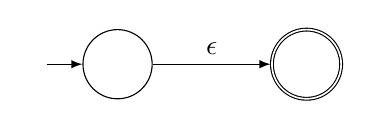
\begin{tikzpicture}[auto, node distance=24mm, initial text=, >=latex]
      \node[state, initial, fill=white]   (q_1) [] {};
      \node[state, accepting, fill=white] (q_2) [right of=q_1] {};

      \path[->] (q_1) edge [] node {$\epsilon$}  (q_2);
  \end{tikzpicture}
\end{center}
If $e = a$, for $a \in \Sigma$, we can make a NFA with a single transition consuming
$a$:
\begin{center}
 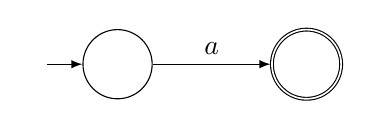
\begin{tikzpicture}[auto, node distance=24mm, initial text=, >=latex]
      \node[state, initial, fill=white]   (q_1) [] {};
      \node[state, accepting, fill=white] (q_2) [right of=q_1] {};

      \path[->] (q_1) edge [] node {$a$}  (q_2);
 \end{tikzpicture}
\end{center}
When $e = e_1 + e_2$, we let $N(e_1)$ be the NFA for $e_1$ and $N(e_2)$ the
NFA for $e_2$. The NFA for $e_1 + e_2$ is built by adding a new initial and accepting
state which can be combined with $N(e_1)$ and $N(e_2)$ using $\epsilon$-transitions as
shown in the next picture.
\begin{center}
    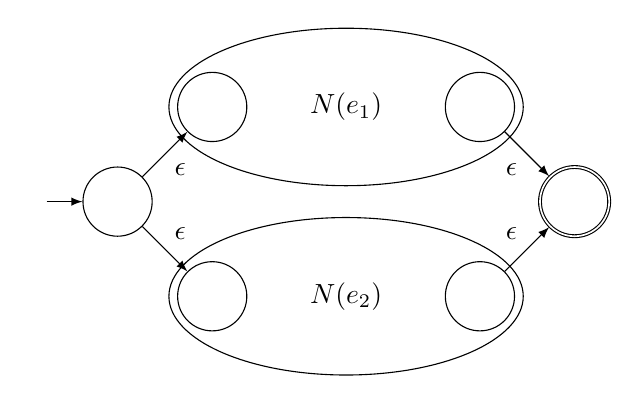
\begin{tikzpicture}[auto, node distance=17mm, initial text=, >=latex]
      \node[state, initial]  (s_i)   []                   {};
      \node[state]        (a_1)   [above right of=s_i] {};
      \node[draw=none,fill=none]            (namea) [right of=a_1] {$N(e_1)$};
      \node[state]         (a_2)   [right of=namea]     {};

      \node[state]        (b_1)   [below right of=s_i] {};
      \node[draw=none]            (nameb) [right of=b_1]           {$N(e_2)$};
      \node[state]         (b_2)   [right of=nameb]     {};

      \node[state, accepting] (s_a)   [below right of=a_2] {};

      \path[->] (s_i) edge [below right] node {$\epsilon$} (a_1)
                      edge [above right] node {$\epsilon$} (b_1)
                (a_2) edge [below left]  node {$\epsilon$} (s_a)
                (b_2) edge []            node {$\epsilon$} (s_a);
      \begin{scope}[on background layer]
        \node[ellipse, draw=black, aspect=5, minimum width=45mm, minimum height=20mm, right of=b_1] {};
        \node[ellipse, draw=black, aspect=5, minimum width=45mm, minimum height=20mm, right of=a_1] {};
      \end{scope}
    \end{tikzpicture}
\end{center}
The NFA for the concatenation $e = e_1e_2$ is built from the NFAs $N(e_1)$ and $N(e_2)$. The accepting
state of $N(e_1e_2)$ will be the accepting state from $N(e_2)$ and the starting state of $N(e_1)$ will be
the initial state of $N(e_1)$.

\begin{center}
    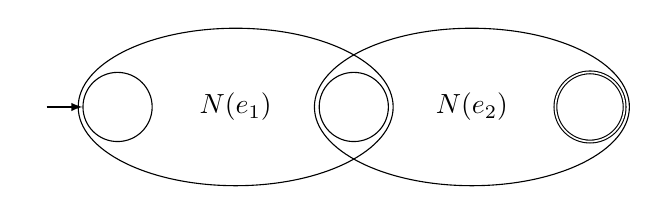
\begin{tikzpicture}[auto,  node distance=15mm, initial text=, >=latex]
      \node[state, initial]   (a_1)   []               {};
      \node[draw=none,fill=none]             (namea) [right of=a_1]   {$N(e_1)$};
      \node[state] (a_2)   [right of=namea] {};

      \node[draw=none]             (nameb) [right of=a_2]   {$N(e_2)$};
      \node[state, accepting]  (b_2)   [right of=nameb] {};

      \begin{scope}[on background layer]
        \node[ellipse, draw=black, aspect=5, minimum width=40mm, minimum height=20mm, right of=a_1] {};
        \node[ellipse, draw=black, aspect=5, minimum width=40mm, minimum height=20mm, right of=a_2] {};
      \end{scope}
    \end{tikzpicture}
\end{center}
Finally, for the Kleene star operator, we built a NFA for the RE $e$, add a new
starting and accepting states and the necessary $\epsilon$ transitions, as shown below.
\begin{center}
    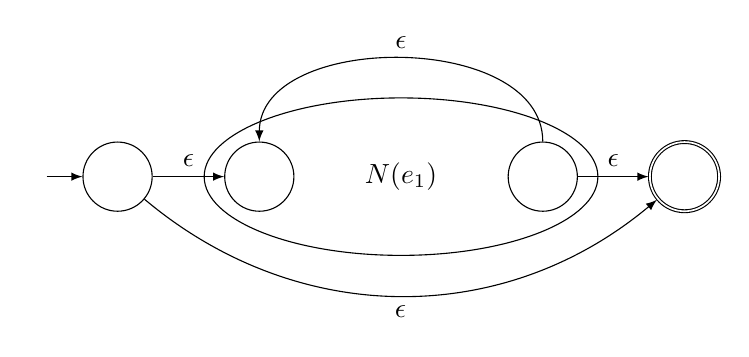
\begin{tikzpicture}[auto, node distance=18mm, initial text=, >=latex]
      \node[state, initial]  (s_i)   []               {};
      \node[state]        (a_1)   [right of=s_i]   {};
      \node[draw=none]            (namea) [right of=a_1]   {$N(e_1)$};
      \node[state]         (a_2)   [right of=namea] {};

      \node[state, accepting] (s_a)   [right of=a_2]   {};

      \path[->] (s_i) edge []                     node {$\epsilon$} (a_1)
                      edge [bend right=40, below] node {$\epsilon$} (s_a)
                (a_2) edge []                     node {$\epsilon$} (s_a)
                      edge [bend right=90, above] node {$\epsilon$} (a_1);
      \begin{scope}[on background layer]
        \node[ellipse, draw=black, aspect=5, minimum width=50mm, minimum height=20mm, right of=a_1] {};
      \end{scope}
    \end{tikzpicture}
\end{center}
Originally, Thompson formulate its construction as a IBM 7094 program~\cite{Thompson1968}. Next we reformulate it as a small-step
operational semantics using contexts, modelled as data-type derivatives for RE, which is the subject of
the next section.

\subsection{Data-type derivatives}

The usage of evaluation contexts is standard in reduction semantics~\cite{Felleisen2009}.
Contexts for evaluating a RE during the parse of a string $s$ can be defined by the following
context-free syntax:
\[E[\,] \to E[\,]+ e\,\mid\,e + E[\,]\,\mid\,E[\,]\,e\,\mid\,e\,E[\,]\,\mid\,\star\]

The semantics of a $E[\,]$ context is a RE with a hole that needs to be ``filled'' to form a
RE. We have two cases for union and concatenation denoting that the hole could be the left
or the right component of such operators. Since the Kleene star has only a recursive occurrence,
it is denoted just as a ``mark'' in context syntax.

Having defined our semantics (Figure~\ref{figure:smallstep}), we have noticed that our RE context syntax is exactly the data type
for \emph{one-hole contexts}, known as derivative of an algebraic data type.
Derivatives where introduced by McBride and its coworkers~\cite{McBride08} as a generalization
of Huet's zippers for a large class of algebraic data types~\cite{AbbottAGM03}. RE contexts are
implemented by the following Haskell data-type:
\begin{hscode}\SaveRestoreHook
\column{B}{@{}>{\hspre}l<{\hspost}@{}}%
\column{3}{@{}>{\hspre}l<{\hspost}@{}}%
\column{E}{@{}>{\hspre}l<{\hspost}@{}}%
\>[B]{}\mathkw{data}\;\D{Hole}\mathrel{=}\C{InChoiceL}\;\D{Regex}\mid \C{InChoiceR}\;\D{Regex}{}\<[E]%
\\
\>[B]{}\hsindent{3}{}\<[3]%
\>[3]{}\mid \C{InCatL}\;\D{Regex}\mid \C{InCatR}\;\D{Regex}\mid \C{InStar}{}\<[E]%
\ColumnHook
\end{hscode}\resethooks
Constructor \ensuremath{\C{InChoiceL}} store the right component of a union RE (similarly for \ensuremath{\C{InChoiceR}}). We need
to store contexts for union because such information is used to allow backtracking in case of failure.
Constructors \ensuremath{\C{InCatL}} and \ensuremath{\C{InCatR}} store the right (left) component of a concatenation and they are
used to store the next subexpresssions that needed to be evaluated during input string parsing.
Finally, \ensuremath{\C{InStar}} marks that we are currently processing an expression with a Kleene star operator.

\section{Proposed semantics}\label{section:semantics}


In this section we present the definition of an operational semantics for RE parsing which is
equivalent to executing the Thompson's construction NFA over the input string. Observe that,
the inductive semantics for RE (Figure~\ref{figure:resemantics}) can be understood as a big-step
operational semantics for RE, since it ignores many details on how should we proceed to match
an input~\cite{Rathnayake2011}.

The semantics is defined as a binary relation between \emph{configurations}, which are 5-uples
$\conf{d,e,c,b,s}$ where:
\begin{itemize}
  \item $d$ is a direction, which specifies if the semantics is starting (denoted by $B$) or
        finishing ($F$) the processing of the current expression $e$.
  \item $e$ is the current expression being evaluated;
  \item $c$ is a context in which $e$ occurs. Contexts are just a list of
        \ensuremath{\D{Hole}} type in our implementation.
  \item $b$ is a bit-code for the current parsing result, in reverse order.
  \item $s$ is the input string currently being processed.
\end{itemize}
Notation $\conf{d,e,c,b,s}\to\conf{d',e',c',b',s'}$ denotes that from
configuration $\conf{d,e,c,b,s}$ we can give a step leading to a new state
$\conf{d',e',c',b',s'}$ using the rules specified in Figure~\ref{figure:smallstep}.

\begin{figure*}[h]
  \[
     \begin{array}{ccc}
        \infer[_{(Eps)}]{\conf{B,\epsilon,c,b,s} \to \conf{F,\epsilon,c,b,s}}{}
        &
        \infer[_{(Chr)}]{\conf{B,a,c,b,a:s} \to \conf{F,a,c,b,s}}{}
        &
        \infer[_{(Left_B)}]{\conf{B,e+e',c,b,s}\to\conf{B,e,c',b',s}}
              {\begin{array}{c}
                 b' = \ensuremath{\C{0_b}} : b\\
                 c' = E[\,]+e' : c \\
               \end{array}}
        \\ \\
        \infer[_{(Right_B)}]{\conf{B,e+e',c,b,s}\to\conf{B,e',c',b',s}}
              {\begin{array}{c}
                 b' = \ensuremath{\C{1_b}} : b\\
                 c' = e + E[\,] : c \\
               \end{array}}
        &
        \infer[_{(Cat_B)}]{\conf{B,ee',c,b,s}\to\conf{B,e,c',b,s}}
              {c' = E[\,]e' : c}
        &
        \infer[_{(Star_1)}]{\conf{B,e^\star,c,b,s}\to\conf{B,e,\star : c, \ensuremath{\C{0_b}} : b, s}}{}
        \\ \\
        \infer[_{(Star_2)}]{\conf{B,e^\star,c,b,s}\to\conf{F,e^\star, c, \ensuremath{\C{1_b}} : b, s}}{}
        &
        \infer[_{(Cat_{EL})}]{\conf{F,e,E[\,]e':c,b,s}\to\conf{B,e',c',b,s}}{c'=eE[\,]:c}
        &
        \infer[_{(Cat_{ER})}]{\conf{F,e',eE[\,]:c,b,s}\to\conf{F,ee',c,b,s}}{}
        \\ \\
        \multicolumn{3}{c}{
            \begin{array}{cc}
               \infer[_{(Left_E)}]{\conf{F,e,c,b,s}\to\conf{F,e+e',c',\ensuremath{\C{0_b}}:b,s}}{c = E[\,]+e' : c'}
            &
               \infer[_{(Right_E)}]{\conf{F,e,c,b,s}\to\conf{F,e+e',c',\ensuremath{\C{1_b}}:b,s}}{c = e + E[\,] : c'}
            \end{array}}
        \\ \\
        \multicolumn{3}{c}{
           \begin{array}{cc}
              \infer[_{(Star_{E1})}]{\conf{F,e,\star:c,b,s}\to\conf{B,e,\star:c,\ensuremath{\C{0_b}}:b,s}}{}
              &
              \infer[_{(Star_{E2})}]{\conf{F,e,\star:c,b,s}\to\conf{F,e^\star,c,\ensuremath{\C{1_b}}:b,s}}{}
           \end{array}
        }
     \end{array}
  \]
  \centering
  \caption{Small-step semantics for RE parsing.}
  \label{figure:smallstep}
\end{figure*}
The rules of the semantics can be divided in two groups: starting rules and finishing rules.
Starting rules deal with configurations with a begin ($B$) direction and denote that we are
beginning the parsing for its RE $e$. Finishing rules use the context to decide how the parsing
for some expression should end. Intuitively, starting rules correspond to transitions entering a
sub-automata of Thompson NFA and finishing rules to transitions exiting a sub-automata.

The meaning of each starting rule is as follows. Rule $\{Eps\}$ specifies that we can mark a state as
finished if it consists of a starting configuration with RE $\epsilon$. We can finish any configuration
for \ensuremath{\C{Chr}\;\V{a}} if it is starting with current string with a leading $a$. Whenever we have a starting configuration
with a choice RE, $e_1 + e_2$, we can non-deterministicaly choose if input string $s$ can be processed by
$e_1$ (rule $Left_B$) or $e_2$ (rule $Right_B$). For beginning configurations with concatenation, we parse
input string using each of its components sequentially. Finally, for starting configurations with a Kleene
star operator, $e^\star$, we can either start the processing of $e$ or finish the processing for $e^\star$.
In all recursive cases for RE, we insert context information in the third component of the resulting
configuration in order to decide how the machine should step after finishing the execution of the RE
currently on focus.

Rule $(Cat_{EL})$ applies to any configuration which is finishing with a left concatenation context ($E[\,]e'$).
In such situation, rule specifies that a computation should continue with $e'$ and push the context $e\,E[\,]$.
We end the computation for a concatenation, whenever we find a context $e\,E[\,]$ in the context component
(rule $(Cat_{ER})$). Finishing a computation for choice consists in just popping its correspondent context,
as done by rules $(Left_E)$ and $(Right_E)$. For the Kleene star operator, we can either finish the computation
by popping the contexts and adding the corresponding \ensuremath{\C{1_b}} to end its matching list or restart with RE $e$ for
another matching over the input string.

The starting state of the semantics is given by the configuration
$\conf{B,e,[],[],s}$ and accepting configurations are $\conf{F,e',[],bs,[]}$, for some RE $e'$ and code $bs$.
Following common practice, we let $\to^\star$ denote the reflexive, transtive closure of the small-step
semantics defined in Figure~\ref{figure:smallstep}.
We say that a string $s$ is accepted by RE $e$ if $\conf{B,e,[],[],s}\to^\star\conf{F,e',[],bs,[]}$.
The next theorem asserts that our semantics is sound and complete with respect to RE
inductive semantics (Figure~\ref{figure:resemantics}).

\begin{Theorem}
   For all strings $s$ and non-problematic REs $e$, $s\in\sembrackets{e}$ if, and only if, $\conf{B,e,[],[],s}\to^\star\conf{F,e',[],b,[]}$ and
   $\conf{F,e',[],b,[]}$ is an accepting configuration.
\end{Theorem}

\section{Implementation details}\label{section:implementation}


In order to implement the small-step semantics of Figure~\ref{figure:smallstep}, we need to represent configurations.
We use type \ensuremath{\D{Conf}} to denote configurations and directions are represented by type \ensuremath{\D{Dir}}, where \ensuremath{\C{Begin}} denote the
starting and \ensuremath{\C{End}} the finishing direction.

\begin{hscode}\SaveRestoreHook
\column{B}{@{}>{\hspre}l<{\hspost}@{}}%
\column{E}{@{}>{\hspre}l<{\hspost}@{}}%
\>[B]{}\mathkw{data}\;\D{Dir}\mathrel{=}\C{Begin}\mid \C{End}{}\<[E]%
\\
\>[B]{}\mathkw{type}\;\D{Conf}\mathrel{=}(\D{Dir},\D{Regex},[\mskip1.5mu \D{Hole}\mskip1.5mu],\D{Code},\D{String}){}\<[E]%
\ColumnHook
\end{hscode}\resethooks

Function \ensuremath{\F{finish}} tests if a configuration is an accepting one.

\begin{hscode}\SaveRestoreHook
\column{B}{@{}>{\hspre}l<{\hspost}@{}}%
\column{E}{@{}>{\hspre}l<{\hspost}@{}}%
\>[B]{}\F{finish}\mathbin{::}\D{Conf}\to \D{Bool}{}\<[E]%
\\
\>[B]{}\F{finish}\;(\C{End},\anonymous ,[\mskip1.5mu \mskip1.5mu],\anonymous ,[\mskip1.5mu \mskip1.5mu])\mathrel{=}\C{True}{}\<[E]%
\\
\>[B]{}\F{finish}\;\anonymous \mathrel{=}\C{False}{}\<[E]%
\ColumnHook
\end{hscode}\resethooks


The small-step semantics is implemented by function \ensuremath{\F{next}}, which returns a list of configurations that can
be reached from a given input configuration. We will begin by explaining the equations that code the set of
starting rules from the small-step semantics. The first alternative

\begin{hscode}\SaveRestoreHook
\column{B}{@{}>{\hspre}l<{\hspost}@{}}%
\column{E}{@{}>{\hspre}l<{\hspost}@{}}%
\>[B]{}\F{next}\mathbin{::}\D{Conf}\to [\mskip1.5mu \D{Conf}\mskip1.5mu]{}\<[E]%
\\
\>[B]{}\F{next}\;(\C{Begin},\C{\epsilon},\V{ctx},\V{bs},\V{s})\mathrel{=}[\mskip1.5mu (\C{End},\C{\epsilon},\V{ctx},\V{bs},\V{s})\mskip1.5mu]{}\<[E]%
\ColumnHook
\end{hscode}\resethooks
implements rule $(Eps)$, which finishes a starting \ensuremath{\D{Conf}} with an \ensuremath{\C{\epsilon}}. Rule $(Chr)$ is implemented by
the following equation
\begin{hscode}\SaveRestoreHook
\column{B}{@{}>{\hspre}l<{\hspost}@{}}%
\column{3}{@{}>{\hspre}l<{\hspost}@{}}%
\column{15}{@{}>{\hspre}l<{\hspost}@{}}%
\column{E}{@{}>{\hspre}l<{\hspost}@{}}%
\>[B]{}\F{next}\;(\C{Begin},\C{Chr}\;\V{c},\V{ctx},\V{bs},\V{a}\mathbin{:}\V{s}){}\<[E]%
\\
\>[B]{}\hsindent{3}{}\<[3]%
\>[3]{}\mid \V{a}\equiv \V{c}\mathrel{=}{}\<[15]%
\>[15]{}[\mskip1.5mu (\C{End},\C{Chr}\;\V{c},\V{ctx},\V{bs},\V{s})\mskip1.5mu]{}\<[E]%
\\
\>[B]{}\hsindent{3}{}\<[3]%
\>[3]{}\mid \F{otherwise}\mathrel{=}[\mskip1.5mu \mskip1.5mu]{}\<[E]%
\ColumnHook
\end{hscode}\resethooks
which consumes input character \ensuremath{\V{a}} if it matches RE \ensuremath{\C{Chr}\;\V{c}}, otherwise it fails by returning an empty list.
For a choice expression, we can use two distinct rules: one for parsing the input using its left component and
another rule for the right. Since both union and Kleene star introduce non-determinism in RE parsing, we can
easily model this using the list monad, by return a list of possible resulting configurations.
\begin{hscode}\SaveRestoreHook
\column{B}{@{}>{\hspre}l<{\hspost}@{}}%
\column{3}{@{}>{\hspre}l<{\hspost}@{}}%
\column{5}{@{}>{\hspre}l<{\hspost}@{}}%
\column{E}{@{}>{\hspre}l<{\hspost}@{}}%
\>[B]{}\F{next}\;(\C{Begin},\V{e}\C{\:+\:}\V{e'},\V{ctx},\V{bs},\V{s}){}\<[E]%
\\
\>[B]{}\hsindent{3}{}\<[3]%
\>[3]{}\mathrel{=}[\mskip1.5mu (\C{Begin},\V{e},\C{InChoiceL}\;\V{e'}\mathbin{:}\V{ctx},\C{0_b}\mathbin{:}\V{bs},\V{s}){}\<[E]%
\\
\>[3]{}\hsindent{2}{}\<[5]%
\>[5]{},(\C{Begin},\V{e'},\C{InChoiceR}\;\V{e}\mathbin{:}\V{ctx},\C{1_b}\mathbin{:}\V{bs},\V{s})\mskip1.5mu]{}\<[E]%
\ColumnHook
\end{hscode}\resethooks
Concatenation just sequences the computation of each of its composing RE.
\begin{hscode}\SaveRestoreHook
\column{B}{@{}>{\hspre}l<{\hspost}@{}}%
\column{3}{@{}>{\hspre}l<{\hspost}@{}}%
\column{E}{@{}>{\hspre}l<{\hspost}@{}}%
\>[B]{}\F{next}\;(\C{Begin},\V{e}\C{\:\bullet\:}\V{e'},\V{ctx},\V{bs},\V{s}){}\<[E]%
\\
\>[B]{}\hsindent{3}{}\<[3]%
\>[3]{}\mathrel{=}[\mskip1.5mu (\C{Begin},\V{e},\C{InCatL}\;\V{e'}\mathbin{:}\V{ctx},\V{bs},\V{s})\mskip1.5mu]{}\<[E]%
\ColumnHook
\end{hscode}\resethooks
For a starting configuration with Kleene star operator, \ensuremath{\C{Star}\;\V{e}}, we can proceed in two ways: by beginning the
parsing of RE \ensuremath{\V{e}} or by finishing the computation for \ensuremath{\C{Star}\;\V{e}} over the input.
\begin{hscode}\SaveRestoreHook
\column{B}{@{}>{\hspre}l<{\hspost}@{}}%
\column{3}{@{}>{\hspre}l<{\hspost}@{}}%
\column{5}{@{}>{\hspre}l<{\hspost}@{}}%
\column{E}{@{}>{\hspre}l<{\hspost}@{}}%
\>[B]{}\F{next}\;(\C{Begin},\C{Star}\;\V{e},\V{ctx},\V{bs},\V{s}){}\<[E]%
\\
\>[B]{}\hsindent{3}{}\<[3]%
\>[3]{}\mathrel{=}[\mskip1.5mu (\C{Begin},\V{e},\C{InStar}\mathbin{:}\V{ctx},\C{0_b}\mathbin{:}\V{bs},\V{s}){}\<[E]%
\\
\>[3]{}\hsindent{2}{}\<[5]%
\>[5]{},(\C{End},(\C{Star}\;\V{e}),\V{ctx},\C{1_b}\mathbin{:}\V{bs},\V{s})\mskip1.5mu]{}\<[E]%
\ColumnHook
\end{hscode}\resethooks
The remaining equations of \ensuremath{\F{next}} deal with operational semantics finishing rules. The equation below implements
rule $(Cat_{EL})$ which specifies that an ended computation for the left component of a concatenation should continue
with its right component.
\begin{hscode}\SaveRestoreHook
\column{B}{@{}>{\hspre}l<{\hspost}@{}}%
\column{3}{@{}>{\hspre}l<{\hspost}@{}}%
\column{E}{@{}>{\hspre}l<{\hspost}@{}}%
\>[B]{}\F{next}\;(\C{End},\V{e},\C{InCatL}\;\V{e'}\mathbin{:}\V{ctx},\V{bs},\V{s}){}\<[E]%
\\
\>[B]{}\hsindent{3}{}\<[3]%
\>[3]{}\mathrel{=}[\mskip1.5mu (\C{Begin},\V{e'},\C{InCatR}\;\V{e}\mathbin{:}\V{ctx},\V{bs},\V{s})\mskip1.5mu]{}\<[E]%
\ColumnHook
\end{hscode}\resethooks
Whenever we are in a finishing configuration with a right concatenation context, (\ensuremath{\C{InCatR}\;\V{e}}), we end the parsing of
the input for the whole concatenation RE.
\begin{hscode}\SaveRestoreHook
\column{B}{@{}>{\hspre}l<{\hspost}@{}}%
\column{3}{@{}>{\hspre}l<{\hspost}@{}}%
\column{E}{@{}>{\hspre}l<{\hspost}@{}}%
\>[B]{}\F{next}\;(\C{End},\V{e'},\C{InCatR}\;\V{e}\mathbin{:}\V{ctx},\V{bs},\V{s}){}\<[E]%
\\
\>[B]{}\hsindent{3}{}\<[3]%
\>[3]{}\mathrel{=}[\mskip1.5mu (\C{End},\V{e}\C{\:\bullet\:}\V{e'},\V{ctx},\V{bs},\V{s})\mskip1.5mu]{}\<[E]%
\ColumnHook
\end{hscode}\resethooks
Next equations implement the rules that finish configurations for the union, by commiting to its first successful branch.
\begin{hscode}\SaveRestoreHook
\column{B}{@{}>{\hspre}l<{\hspost}@{}}%
\column{3}{@{}>{\hspre}l<{\hspost}@{}}%
\column{E}{@{}>{\hspre}l<{\hspost}@{}}%
\>[B]{}\F{next}\;(\C{End},\V{e},\C{InChoiceL}\;\V{e'}\mathbin{:}\V{ctx},\V{bs},\V{s}){}\<[E]%
\\
\>[B]{}\hsindent{3}{}\<[3]%
\>[3]{}\mathrel{=}[\mskip1.5mu (\C{End},\V{e}\C{\:+\:}\V{e'},\V{ctx},\C{0_b}\mathbin{:}\V{bs},\V{s})\mskip1.5mu]{}\<[E]%
\\
\>[B]{}\F{next}\;(\C{End},\V{e'},\C{InChoiceR}\;\V{e}\mathbin{:}\V{ctx},\V{bs},\V{s}){}\<[E]%
\\
\>[B]{}\hsindent{3}{}\<[3]%
\>[3]{}\mathrel{=}[\mskip1.5mu (\C{End},\V{e}\C{\:+\:}\V{e'},\V{ctx},\C{1_b}\mathbin{:}\V{bs},\V{s})\mskip1.5mu]{}\<[E]%
\ColumnHook
\end{hscode}\resethooks
Equations for Kleene star implement rules $(Star_{E1})$ and $(Star_{E2})$ which allows ending or add one more match
for an RE $e$.
\begin{hscode}\SaveRestoreHook
\column{B}{@{}>{\hspre}l<{\hspost}@{}}%
\column{3}{@{}>{\hspre}l<{\hspost}@{}}%
\column{5}{@{}>{\hspre}l<{\hspost}@{}}%
\column{E}{@{}>{\hspre}l<{\hspost}@{}}%
\>[B]{}\F{next}\;(\C{End},\V{e},\C{InStar}\mathbin{:}\V{ctx},\V{bs},\V{s}){}\<[E]%
\\
\>[B]{}\hsindent{3}{}\<[3]%
\>[3]{}\mathrel{=}[\mskip1.5mu (\C{Begin},\V{e},\C{InStar}\mathbin{:}\V{ctx},\C{0_b}\mathbin{:}\V{bs},\V{s}){}\<[E]%
\\
\>[3]{}\hsindent{2}{}\<[5]%
\>[5]{},(\C{End},(\C{Star}\;\V{e}),\V{ctx},\C{1_b}\mathbin{:}\V{bs},\V{s})\mskip1.5mu]{}\<[E]%
\ColumnHook
\end{hscode}\resethooks
Finally, stuck states on the semantics are properly handled by the following equation which turns them all
into a failure (empty list).
\begin{hscode}\SaveRestoreHook
\column{B}{@{}>{\hspre}l<{\hspost}@{}}%
\column{E}{@{}>{\hspre}l<{\hspost}@{}}%
\>[B]{}\F{next}\;\anonymous \mathrel{=}[\mskip1.5mu \mskip1.5mu]{}\<[E]%
\ColumnHook
\end{hscode}\resethooks
The reflexive-transitive closure of the semantics is implemented by function \ensuremath{\F{steps}}, which computes the
trace of all states needed to determine if a string can be parsed by the RE $e$.
\begin{hscode}\SaveRestoreHook
\column{B}{@{}>{\hspre}l<{\hspost}@{}}%
\column{E}{@{}>{\hspre}l<{\hspost}@{}}%
\>[B]{}\F{steps}\mathbin{::}[\mskip1.5mu \D{Conf}\mskip1.5mu]\to [\mskip1.5mu \D{Conf}\mskip1.5mu]{}\<[E]%
\\
\>[B]{}\F{steps}\;[\mskip1.5mu \mskip1.5mu]\mathrel{=}[\mskip1.5mu \mskip1.5mu]{}\<[E]%
\\
\>[B]{}\F{steps}\;\V{cs}\mathrel{=}\F{steps}\;[\mskip1.5mu \V{c'}\mid \V{c}\leftarrow \V{cs},\V{c'}\leftarrow \F{next}\;\V{c}\mskip1.5mu]\plus \V{cs}{}\<[E]%
\ColumnHook
\end{hscode}\resethooks
Finally, the function for parsing a string using an input RE is implemented as follows:
\begin{hscode}\SaveRestoreHook
\column{B}{@{}>{\hspre}l<{\hspost}@{}}%
\column{15}{@{}>{\hspre}l<{\hspost}@{}}%
\column{17}{@{}>{\hspre}l<{\hspost}@{}}%
\column{E}{@{}>{\hspre}l<{\hspost}@{}}%
\>[B]{}\F{vmAccept}\mathbin{::}\D{String}\to \D{Regex}\to (\D{Bool},\D{Code}){}\<[E]%
\\
\>[B]{}\F{vmAccept}\;\V{s}\;\V{e}\mathrel{=}\mathkw{let}\;\V{r}\mathrel{=}[\mskip1.5mu \V{c}\mid \V{c}\leftarrow \F{steps}\;\F{init_{cfg}},\F{finish}\;\V{c}\mskip1.5mu]{}\<[E]%
\\
\>[B]{}\hsindent{15}{}\<[15]%
\>[15]{}\mathkw{in}\;\mathkw{if}\;\F{null}\;\V{r}\;\mathkw{then}\;(\C{False},[\mskip1.5mu \mskip1.5mu])\;\mathkw{else}\;(\C{True},\F{bitcode}\;(\F{head}\;\V{r})){}\<[E]%
\\
\>[B]{}\hsindent{15}{}\<[15]%
\>[15]{}\mathkw{where}{}\<[E]%
\\
\>[15]{}\hsindent{2}{}\<[17]%
\>[17]{}\F{init_{cfg}}\mathrel{=}[\mskip1.5mu (\C{Begin},\V{e},[\mskip1.5mu \mskip1.5mu],[\mskip1.5mu \mskip1.5mu],\V{s})\mskip1.5mu]{}\<[E]%
\\
\>[15]{}\hsindent{2}{}\<[17]%
\>[17]{}\F{bitcode}\;(\anonymous ,\anonymous ,\anonymous ,\V{bs},\anonymous )\mathrel{=}\F{reverse}\;\V{bs}{}\<[E]%
\ColumnHook
\end{hscode}\resethooks
Function \ensuremath{\F{vmAccept}} returns a pair formed by a boolean and the bit-code produced during the parsing of
an input string and RE. Observe that, we need to reverse the bit-codes, since they are built in reverse
order.

\subsection{Test suite}

\paragraph{An overview of QuickCheck.}
Our tests are implemented using QuickCheck~\cite{Claessen2000}, a library
that allows the testing of properties expressed as Haskell functions.
Such verification is done by generating random values of the desired type,
instantiating the relevant property with them, and checking it directly by
evaluating it to a boolean. This process continues until a counterexample is
found or a specified number of cases are tested with success.
The library provides generators for several standard library
data types and combinators to build new generators for user-defined
types.


As an example of a custom generator, consider the task of generating a
random alpha-numeric character. To implement such generator, \ensuremath{\F{genChar}}, we
use QuickCheck function \ensuremath{\F{suchThat}} which generates a random value with satisfies
a predicate passed as argument (in example, we use \ensuremath{\F{isAlphaNum}} which is true whenever
we pass an alpha-numeric character to it), using an random generator taken as input.

\begin{hscode}\SaveRestoreHook
\column{B}{@{}>{\hspre}l<{\hspost}@{}}%
\column{E}{@{}>{\hspre}l<{\hspost}@{}}%
\>[B]{}\F{genChar}\mathbin{::}\D{Gen}\;\D{Char}{}\<[E]%
\\
\>[B]{}\F{genChar}\mathrel{=}\F{suchThat}\;(\F{arbitrary}\mathbin{::}\D{Gen}\;\D{Char})\;\F{isAlphaNum}{}\<[E]%
\ColumnHook
\end{hscode}\resethooks


\paragraph{Test case generators.} In order to test the correctness of our semantics, we needed to
build generators for REs and for strings. We develop functions to randomly generate strings accepted
and rejected for a RE, using the QuickCheck library.

Generation of random RE is done by function \ensuremath{\F{sizedRegex}} with takes a depth limit to restrict
the size of the generated RE. Whenever the input depth limit is less or equal to 1, we can
only build a \ensuremath{\C{\epsilon}} or a single character RE. The definition of \ensuremath{\F{sizedRegex}} uses
QuickCheck function \ensuremath{\F{frequency}}, which receives a list of pairs formed by a weight and
a random generator and produce, as result, a generator which uses such frequency distribution.
In \ensuremath{\F{sizedRegex}} implementation we give a higher weight to generate characters and equal distributions
to build concatenation, union or star.

\begin{hscode}\SaveRestoreHook
\column{B}{@{}>{\hspre}l<{\hspost}@{}}%
\column{3}{@{}>{\hspre}l<{\hspost}@{}}%
\column{10}{@{}>{\hspre}l<{\hspost}@{}}%
\column{23}{@{}>{\hspre}l<{\hspost}@{}}%
\column{E}{@{}>{\hspre}l<{\hspost}@{}}%
\>[B]{}\F{sizedRegex}\mathbin{::}\D{Int}\to \D{Gen}\;\D{Regex}{}\<[E]%
\\
\>[B]{}\F{sizedRegex}\;\V{n}{}\<[E]%
\\
\>[B]{}\hsindent{3}{}\<[3]%
\>[3]{}\mid \V{n}\leq \C{1}\mathrel{=}\F{frequency}\;[\mskip1.5mu (\C{10},\F{return}\;\C{\epsilon}),(\C{90},\C{Chr}\F{\,\langle\$\rangle\,}\F{genChar})\mskip1.5mu]{}\<[E]%
\\
\>[B]{}\hsindent{3}{}\<[3]%
\>[3]{}\mid \F{otherwise}\mathrel{=}\F{frequency}\;[\mskip1.5mu (\C{10},\F{return}\;\C{\epsilon}),(\C{30},\C{Chr}\F{\,\langle\$\rangle\,}\F{genChar}){}\<[E]%
\\
\>[3]{}\hsindent{7}{}\<[10]%
\>[10]{},(\C{20},(\C{\:\bullet\:})\F{\,\langle\$\rangle\,}\F{sizedRegex}\;\V{n2}\F{\,\langle\star\rangle\,}\F{sizedRegex}\;\V{n2}){}\<[E]%
\\
\>[3]{}\hsindent{7}{}\<[10]%
\>[10]{},(\C{20},(\C{\:+\:})\F{\,\langle\$\rangle\,}\F{sizedRegex}\;\V{n2}\F{\,\langle\star\rangle\,}\F{sizedRegex}\;\V{n2}){}\<[E]%
\\
\>[3]{}\hsindent{7}{}\<[10]%
\>[10]{},(\C{20},\C{Star}{}\<[23]%
\>[23]{}\F{\,\langle\$\rangle\,}\F{suchThat}\;(\F{sizedRegex}\;\V{n2})\;(\F{not}\mathbin{\circ}\F{nullable}))\mskip1.5mu]{}\<[E]%
\\
\>[3]{}\hsindent{7}{}\<[10]%
\>[10]{}\mathkw{where}\;\V{n2}\mathrel{=}\F{div}\;\V{n}\;\C{2}{}\<[E]%
\ColumnHook
\end{hscode}\resethooks


Given an RE \ensuremath{\V{e}}, we can generate a random string $s$ such that $s \in\sembrackets{e}$
using the next definition. We generate strings by choosing randomly between branches of
a union or by repeating $n$ times a string $s$ which is accepted by $e$, whenever we
have $e^\star$ (function \ensuremath{\F{randomMatches}}).

\begin{hscode}\SaveRestoreHook
\column{B}{@{}>{\hspre}l<{\hspost}@{}}%
\column{3}{@{}>{\hspre}l<{\hspost}@{}}%
\column{7}{@{}>{\hspre}l<{\hspost}@{}}%
\column{29}{@{}>{\hspre}l<{\hspost}@{}}%
\column{38}{@{}>{\hspre}l<{\hspost}@{}}%
\column{E}{@{}>{\hspre}l<{\hspost}@{}}%
\>[B]{}\F{randomMatch}\mathbin{::}\D{Regex}\to \D{Gen}\;\D{String}{}\<[E]%
\\
\>[B]{}\F{randomMatch}\;\C{\epsilon}\mathrel{=}\F{return}\;\text{\tt \char34 \char34}{}\<[E]%
\\
\>[B]{}\F{randomMatch}\;(\C{Chr}\;\V{c})\mathrel{=}\F{return}\;[\mskip1.5mu \V{c}\mskip1.5mu]{}\<[E]%
\\
\>[B]{}\F{randomMatch}\;(\V{e}\C{\:\bullet\:}\V{e'})\mathrel{=}\F{liftM2}\;(\plus )\;(\F{randomMatch}\;\V{e})\;{}\<[E]%
\\
\>[B]{}\hsindent{38}{}\<[38]%
\>[38]{}(\F{randomMatch}\;\V{e'}){}\<[E]%
\\
\>[B]{}\F{randomMatch}\;(\V{e}\C{\:+\:}\V{e'})\mathrel{=}\F{oneof}\;[\mskip1.5mu \F{randomMatch}\;\V{e},\F{randomMatch}\;\V{e'}\mskip1.5mu]{}\<[E]%
\\
\>[B]{}\F{randomMatch}\;(\C{Star}\;\V{e})\mathrel{=}\mathkw{do}{}\<[E]%
\\
\>[B]{}\hsindent{7}{}\<[7]%
\>[7]{}\V{n}\leftarrow \F{choose}\;(\C{0},\C{3})\mathbin{::}\D{Gen}\;\D{Int}{}\<[E]%
\\
\>[B]{}\hsindent{7}{}\<[7]%
\>[7]{}\F{randomMatches}\;\V{n}\;\V{e}{}\<[E]%
\\[\blanklineskip]%
\>[B]{}\F{randomMatches}\mathbin{::}\D{Int}\to \D{Regex}\to \D{Gen}\;\D{String}{}\<[E]%
\\
\>[B]{}\F{randomMatches}\;\V{m}\;\V{e'}{}\<[E]%
\\
\>[B]{}\hsindent{3}{}\<[3]%
\>[3]{}\mid \V{m}\leq \C{0}\mathrel{=}\F{return}\;[\mskip1.5mu \mskip1.5mu]{}\<[E]%
\\
\>[B]{}\hsindent{3}{}\<[3]%
\>[3]{}\mid \F{otherwise}\mathrel{=}\F{liftM2}\;(\plus )\;(\F{randomMatch}\;\V{e'})\;{}\<[E]%
\\
\>[3]{}\hsindent{26}{}\<[29]%
\>[29]{}(\F{randomMatches}\;(\V{m}\mathbin{-}\C{1})\;\V{e'}){}\<[E]%
\ColumnHook
\end{hscode}\resethooks
The algorithm for generating random strings that aren't accepted by a RE is similarly defined
and omitted for brevity.

\paragraph{Properties considered.}


In order to verify if the defined semantics is correct, we need to check the following properties:
\begin{itemize}
   \item Our semantics accepts only and all the strings in the language described by the input RE: we
         test this property by generating random strings that should be accepted and strings that must
         be rejected by a random RE.
   \item Our semantics generates valid parsing evidence: the bit-codes produced as result, have the
         following properties: 1) the bit-codes can be parsed into a valid parse tree $t$ for the random
         produced RE $e$, i.e. $\vdash t : e$ holds ; 2) \ensuremath{\F{flat}\;\V{t}\mathrel{=}\V{s}} and 3) \ensuremath{\F{code}\;\V{e}\;\V{t}\mathrel{=}\V{bs}}.
\end{itemize}
In addition to coding / decoding of parse trees, we need a function which checks if a tree is indeed a
parsing evidence for some RE $e$. Function \ensuremath{\F{tc}} takes, as arguments, a parse tree $t$ and a RE $e$ and
verifies if $t$ is an evidence for $e$.

\begin{hscode}\SaveRestoreHook
\column{B}{@{}>{\hspre}l<{\hspost}@{}}%
\column{E}{@{}>{\hspre}l<{\hspost}@{}}%
\>[B]{}\F{tc}\mathbin{::}\D{Tree}\to \D{Regex}\to \D{Bool}{}\<[E]%
\\
\>[B]{}\F{tc}\;\C{()}\;\C{\epsilon}\mathrel{=}\C{True}{}\<[E]%
\\
\>[B]{}\F{tc}\;(\C{Chr}\;\V{c})\;(\C{Chr}\;\V{c'})\mathrel{=}\V{c}\equiv \V{c'}{}\<[E]%
\\
\>[B]{}\F{tc}\;(\V{t}\C{\:\bullet\:}\V{t'})\;(\V{e}\C{\:\bullet\:}\V{e'})\mathrel{=}\F{tc}\;\V{t}\;\V{e}\mathrel{\wedge}\F{tc}\;\V{t'}\;\V{e'}{}\<[E]%
\\
\>[B]{}\F{tc}\;(\C{InL}\;\V{t})\;(\V{e}\C{\:+\:}\anonymous )\mathrel{=}\F{tc}\;\V{t}\;\V{e}{}\<[E]%
\\
\>[B]{}\F{tc}\;(\C{InR}\;\V{t'})\;(\anonymous \C{\:+\:}\V{e'})\mathrel{=}\F{tc}\;\V{t'}\;\V{e'}{}\<[E]%
\\
\>[B]{}\F{tc}\;(\C{List}\;\V{ts})\;(\C{Star}\;\V{e})\mathrel{=}\F{all}\;(\F{flip}\;\F{tc}\;\V{e})\;\V{ts}{}\<[E]%
\ColumnHook
\end{hscode}\resethooks

Function \ensuremath{\F{tc}} is a implementation of parsing tree typing relation, as specified by the following
result.
\begin{Theorem}
For all tree $t$ and RE $e$, $\vdash t : e$ if, and only if, \ensuremath{\F{tc}\;\V{t}\;\V{e}\mathrel{=}\C{True}}.
\end{Theorem}


\paragraph{Code coverage results.}

After running thousands of well-succeeded tests, we gain a high degree of confidence in the correctness
of our semantics, however, it is important to measure how much of our code is covered by the test suite.
We use the Haskell Program Coverage tool (HPC)~\cite{Gill2007} to generate statistics about the execution of our tests.
Code coverage results are presented in Figure~\ref{figure:coverage}.

\begin{figure}[h!]
  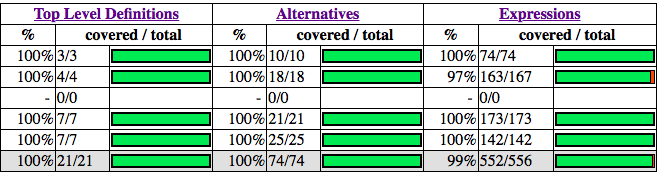
\includegraphics[width=\linewidth]{coverage-results.png}
  \caption{Code coverage results}
  \label{figure:coverage}
\end{figure}

Our test suite give us almost 100\% of code coverage, which provides a strong evidence that our semantics
is indeed correct. All top level definitions and function alternatives are actually executed by the test cases
and just two expressions are marked as non-executed by HPC.

\section{Related work}\label{section:related}

Ierusalimschy \cite{Ierusalimschy2009} proposed the use of Parsing Expression Grammars (PEGs) as a basis
for pattern matching. He argued that pure REs is a weak formalism for pattern-matching tasks:
many interesting patterns either are difficult to to describe or cannot be described by REs. He also said
that the inherent non-determinism of REs does not fit the need to capture specific parts of a match. Following
this proposal, he presented LPEG, a pattern-matching tool based on PEGs for the Lua language. He
argued that LPEG unifies the ease of use of pattern-matching tools with the full expressive power of PEGs.
He also presented a parsing machine (PM) that allows an implementation of PEGs for pattern matching.
In~\cite{Medeiros2008}, Medeiros et. al. presents informal correctness proofs of LPEG PM.
While such proofs represent a important step towards the correctness of LPEG, there is no guarantee that LPEG
implementation follows its specification.

In \cite{Rathnayake2011}, Rathnayake and Thielecke formalized a VM implementation for RE matching using
operational semantics. Specifically, they derived a series of abstract machines, moving from the abstract
definition of matching to realistic machines. First, a continuation is added to the operational semantics
to describe what remains to be matched after the current expression. Next, they represented the expression
as a data structure using pointers, which enables redundant searches to be eliminated via testing for pointer
equality. Although their work has some similarities with ours (a VM-based parsing of REs), they did not present
any evidence or proofs that their VM is correct.

Fischer, Huch and Wilke \cite{Fischer2010} developed a Haskell program for matching REs. The program is purely
functional and it is overloaded over arbitrary semirings, which solves the matching problem and supports other
applications like computing leftmost longest matchings or the number of matchings. Their program can also be used
for parsing every context-free language by taking advantage of laziness. Their developed program is based on an
old technique to turn REs into finite automata, which makes it efficient compared to other similar approaches.
One advantage of their implementation over our proposal is that their approach works with context-free languages,
not only with REs purely. However, they did not present any correctness proofs of their Haskell code.

Cox~\cite{Cox2009} said that viewing RE matching as executing a special machine makes it possible to add new
features just by the inclusion of new machine instructions. He presented two different ways to implement
a VM that executes a RE that has been compiled into  byte-codes: a recursive and a non-recursive
backtracking implementation, both in C programming language. Cox's work on VM-based RE parsing is poorly specified:
both the VM semantics and the RE compilation process are described only informally
and no correctness guarantees is even mentioned.

Frisch and Cardelli~\cite{Frisch2004} studied the theoretical problem of matching a flat sequence against a type (RE): the
result of the process is a structured value of a given type. Their contributions were in noticing that: (1) A disambiguated
result of parsing can be presented as a data structure that does not contain ambiguities. (2) There are problematic cases in
parsing values of star types that need to be disambiguated. (3) The disambiguation strategy used in XDuce and CDuce (two
XML-oriented functional languages) pattern matching can be characterized mathematically by what they call greedy RE matching.
(4) There is a linear time algorithm for the greedy matching. Their approach is different since they want to axiomatize abstractly
the disambiguation policy, without providing an explicit matching algorithm. They identify three notions of problematic words, REs,
and values (which represent the ways to match words), relate these three notions, and propose matching algorithms to deal with the
problematic case.

Ribeiro and Du Bois~\cite{Ribeiro2017} described the formalization of a RE parsing algorithm that produces a bit representation
of its parse tree in the dependently typed language Agda. The algorithm computes bit-codes using Brzozowski derivatives and
they proved that the produced codes are equivalent to parse trees ensuring soundness and completeness with respect to an
inductive RE semantics. They included the certified algorithm in a tool developed by themselves, named verigrep, for RE-based
search in the style of GNU grep. While the authors provide formal proofs, their tool show a bad performance when compared with
other approaches to RE parsing. Besides, they did not prove that their algorithm follows some disambiguation policy, like POSIX
or greedy.

Nielsen and Henglein~\cite{Lasse2011} showed how to generate a compact \textit{bit-coded} representation of a parse tree for a
given RE efficiently, without explicitly constructing the parse tree first, by simplifying the DFA-based parsing algorithm of
Dub\'e and Feeley~\cite{Dube2000} to emit a bit representation without explicitly materializing the parse tree itself.
They also showed that Frisch and Cardelli's greedy RE parsing algorithm \cite{Frisch2004} can be straightforwardly modified to
produce bit codings directly. They implemented both solutions as well as a backtracking parser and performed benchmark experiments
to measure their performance. They argued that bit codings are interesting in their own right since they are typically not
only smaller than the parse tree, but also smaller than the string being parsed and can be combined with other techniques for
improved text compression. As others related works, the authors did not present a formal verification of their implementations.

An algorithm for POSIX RE parsing is described in~\cite{Sulzmann14}. The main idea of the article is to adapt
derivative parsing to construct parse trees incrementally to solve both matching and submatching for REs. In order to improve the
efficiency of the proposed algorithm, Sulzmann et al. use a bit encoded representation of RE parse trees. Textual proofs of
correctness of the proposed algorithm are presented in an appendix.

\section{Conclusion}\label{section:conclusion}

In this work, we presented a small-step operational semantics for a virtual machine for RE parsing inspired on
Thompson's NFA construction. Our semantics produces, as parsing evidence, bit-codes which can be used to characterize which
disambiguation strategy is followed by the semantics. We use data-type derivatives to represent evaluation contexts for RE.
Such contexts are used to decide how to finish the execution of the RE on focus. We have developed a prototype implementation
of our semantics in Haskell and use QuickCheck to verify its relevant properties with respect to a simple implementation
of RE parsing by Fisher et. al.~\cite{Fischer2010}.

Currently, we have a formalized interpreter of our semantics in Coq proof assistant~\cite{Bertot2010} available at project's
on-line repository~\cite{regexvm-rep}. We are working on formalizing the equivalence between the proposed semantics and
the standard RE inductive semantics.

As future work we intend to use our verified semantics to build a certified tool for RE
parsing, work on proofs that the semantics follow a specific disambiguation strategy and investigate how other algorithms
(e.g. the Glushkov construction~\cite{Gluskov1961}) for converting a RE into a finite state machine could be expressed in
terms of an operational semantics.

\vspace{-2.0ex}

\section*{Acknowledgements}

We would like to thank Prof. \emph{Leonardo Vieira}, \emph{Samuel Feitosa} and the the anonymous reviewers for their valuable
suggestions and comments on early versions of this paper.

\vspace{-2.0ex}


\bibliographystyle{ACM-Reference-Format}
\bibliography{references}

\end{document}


\section{Introduction}\label{sec:intro}

We name parsing the process of analyzing if a sequence of symbols matches a given set of rules.
Such rules are usually specified in a formal notation, like a grammar. If a string can be obtained
from those rules, we have success: we can build some evidence that the input is in the language
described by the underlying formalism. Otherwise, we have a failure: no such evidence exists.

In this work, we focus on the parsing problem for regular expressions (REs), which are an algebraic
and compact way of defining regular languages (RLs), i.e., languages that can be recognized by
(non-)deterministic finite automata and equivalent formalisms. REs are widely used in string search
tools, lexical analyser generators and XML schema languages~\cite{Frisch2004}. Since RE parsing
is pervasive in computing, its correctness is crucial. Nowadays, with the recent
development of languages with dependent types and proof assistants it has become
possible to represent algorithmic properties as program types which are verified
by the compiler. The usage of proof assistants to verify RE parsing / matching algorithms
were the subject of study of several recent research works (e.g ~\cite{Firsov13,Ribeiro2017,Lopes2016,Asperti10}).

Approaches for RE parsing can use representations of finite state machines (e.g.~\cite{Firsov13}),
derivatives (e.g.~\cite{Ribeiro2017,Lopes2018,Lopes2016}) or the so-called pointed RE's or its
variants~\cite{Asperti10,Fischer2010}. Another approach for parsing is based on the so-called
parsing machines, which dates back to 70's with Knuth's work
on top-down syntax analysis for context-free languages~\cite{Knuth71}. Recently, some works
have tried to revive the use of such machines for parsing: Cox~\cite{Cox2009} defined a VM
for which a RE can be seen as ``high-level programs'' that can be compiled to a sequence of
such VM instructions and Lua library LPEG~\cite{Ierusalimschy2009} defines a VM whose instruction
set can be used to compile Parser Expressions Grammars (PEGs)~\cite{Ford04}. Such renewed research
interest is motivated by the fact that is possible to include new features by just adding and
implementing new machine instructions.

Since LPEG VM is designed with PEGs in mind, it is not appropriate for RE parsing, since the ``star''
operator for PEGs has a greedy semantics which differs from the conventional RE semantics for this operator. 
Also, Cox's work on VM-based RE parsing has problems. First, it is poorly specified: both the VM semantics 
and the RE compilation process are described only informally and no correctness guarantee is even mentioned. 
Second, it does not provide an evidence for matching, which could be used to characterize a disambiguation 
strategy, like Greedy~\cite{Frisch2004} and POSIX~\cite{Sulzmann14}. To the best of our knowledge, no 
previous work has formally defined a VM for RE parsing that produces evidence (parse trees) for successful matches.
The objective of this work is to give a first step in filling this gap. More specifically, we are interested in formally
specify and prove the correctness of a VM based semantics for RE parsing which produces bit-codes as
a memory efficient representation of parse-trees. As pointed by~\cite{Lasse2011}, bit-codes are useful because they
are not only smaller than the parse tree, but also smaller than the string being parsed and they can be combined with methods
for text compression. We would like to emphasize that, unlike Cox's work, which develops its VM using a instruction 
set like syntax and semantics, we use, as inspiration, virtual machines for the~$\lambda$-calculus, like the 
SECD and Krivine machines~\cite{Krivine07,Landin64}. 

One important issue regarding RE parsing is how to deal with the so-called problematic 
RE\footnote{We say that a RE $e$ is problematic if there's exists $e_1$ s.t. $e = e_1^\star$ and 
$e_1$ accepts the empty string.}\cite{Frisch2004}. In order to avoid the well-known issues with 
problematic RE, we use a transformation proposed by Medeiros et. al.~\cite{Medeiros14} which turns a
problematic RE into an equivalent non-problematic one. We prove that this algorithm indeed produce
equivalent REs using Coq proof assistant.

Our contributions are:

\begin{itemize}
  \item We present a big step semantics for RE parsing VM which produces bit-codes as parsing evidence.
  \item We develop a certified implementation of an algorithm that converts a problematic RE into a 
  non-problematic one.
  \item We prove that the bit-codes produced by our VM are valid parsing evidence.
  \item We extract from our formalization a certified algorithm in Haskell and use it 
  to build a RE parsing tool. We compare its performance against 
  well known Haskell library for RE parsing.  
\end{itemize}

This paper describes the continuation of the RE VM-based parsing research which we previously reported 
on a paper published on SBLP 2018~\cite{Delfino18}. The current work improves our previous results
mainly by: 1) using a big-step operational semantics which deals correctly with problematic REs, unlike
our previous small-step semantics. We simply transform problematic REs into
equivalent non-problematic ones before starting their execution by our semantics;
2) all results of this paper are completely mechanized using Coq
proof assistant. Our previous work used property-based testing in order to provide an evidence for 
the correctness of the small-step semantics.    

The rest of this paper is organized as follows. Section~\ref{section:coq} gives a 
suscint introduction to Coq proof assistant. Section~\ref{section:background} presents some 
background concepts on RE and its parsing problem. 
Our operational semantics for RE parsing and its theoretical properties
are described in Section~\ref{section:semantics}. Our Coq formalization is described in 
Section~\ref{section:formalization}.  Section~\ref{section:experiments} presents some experimental
results regarding the tool produced using the verified algorithm and Section~\ref{section:related} discuss
related works. Finally, Section~\ref{section:conclusion} concludes and 
presents some directions for future work.

While all the code on which this paper is based has been developed in Coq,
we adopt a ``lighter'' syntax when presenting its code fragments. 
We chose this presentation style in order to improve readability, because
 functions that use dependently typed pattern matching require a high number of type
 annotations, which would deviate from our objective of providing an easily
 understandable formalization. For theorems and lemmas, we sketch the proof strategy 
 but omit tactic scripts.

\paragraph{Coq formalization} All source code produced, including the source of this article, 
instructions on how to build it and replicate the reported experiments are avaliable 
on-line~\cite{regexvm-rep}.

\section{A tour of Coq proof assistant}\label{section:coq}

Coq is a proof assistant based on the calculus of inductive
constructions (CIC)~\cite{Bertot2010}, a higher-order typed
$\lambda$-calculus extended with inductive definitions. Theorem
proving in Coq follows the ideas of the so-called
``BHK-correspondence''\footnote{Abbreviation of Brower, Heyting,
  Kolmogorov, de Bruijn and Martin-L\"of Correspondence. This is also
  known as the Curry-Howard ``isomorphism''.}, in which types represent
logical formulas, $\lambda$-terms represent proofs, and the task of
checking if a piece of text is a proof of a given formula corresponds
to type-checking (i.e. checking if the term that represents the proof
has the type corresponding to the given formula)~\cite{Sorensen2006}.

Writing a proof term whose type is that of a logical formula can be
however a hard task, even for simple propositions.  In order to make
this task easier, Coq provides \emph{tactics}, which are commands that
can be used to help the user in the construction of proof terms.

In this section we provide a brief overview of Coq. We start with a
small example, that uses basic
features of Coq --- types, functions and proof definitions.  In this
example, we use an inductive type that represents natural numbers in
Peano notation. The \coq{nat} type definition includes an
annotation, that indicates that it belongs to the \coq{Set}
sort\footnote{Coq's type language classifies new inductive (and
  co-inductive) definitions by using sorts. \coq{Set} is the sort
  of computational values (programs) and \coq{Prop} is the sort of
  logical formulas and proofs.}. Type \coq{nat} is formed by two
data constructors: \coq{O}, that represents the number $0$, and \coq{S},
the successor function.
\begin{minted}{coq}
Inductive nat : Set :=
| O : nat
| S : nat -> nat.

Fixpoint plus (n m : nat) : nat :=
   match n with
   | O => m
   | S n' => S (plus n' m)
   end.

Theorem plus0r : forall n, plus n 0 = n.
Proof.
   intros n. induction n.
   reflexivity.
   simpl. rewrite -> IHn. reflexivity.
Qed.
\end{minted}   

Command \coq{Fixpoint} allows the definition of functions by
structural recursion. The definition of \coq{plus}, for summing two
values of type \coq{nat}, is straightforward. It should be noted
that all functions defined in Coq must be total.

Besides declaring inductive types and functions, Coq allows us to
define and prove theorems. In our example, we show a simple theorem
about \coq{plus}, that states that
\coq{plus n 0 = n}, for an arbitrary value \coq{n} of type
\coq{nat}. Command \coq{Theorem} allows the statement of a
formula that we want to prove and starts the \emph{interactive proof mode}, 
in which tactics can be used to produce the proof term that
is the proof of such formula. In the example, various tactics are
used to prove the desired result.  The first tactic, \coq{intros}, is
used to move premisses and universally quantified variables from the
goal to the hypothesis. Tactic \coq{induction} is used to start an inductive
proof over an inductively defined object (in our example,
the natural number \coq{n}), generating a case for each constructor and
an induction hypothesis for each recursive branch in constructors.
Tactic \coq{reflexivity} proves trivial equalities up to conversion and
\coq{rewrite} is used to replace terms using some equality. 

For each inductively defined data type,
Coq generates automatically an induction principle~\cite[Chapter
14]{Bertot2010}. For natural numbers, the following Coq term, called
\coq{nat_ind}, is created: 
\begin{minted}{coq}
nat_ind
     : forall P : nat -> Prop,
       P O -> (forall n : nat, P n -> P (S n)) ->
       forall n : nat, P n
\end{minted}
It expects a property (\coq{P}) over natural numbers (a value of type
\coq{nat -> Prop}), a proof that \coq{P} holds for zero (a value of
type \coq{P 0}) and a proof that if \coq{P} holds for an arbitrary
natural \coq{n}, then it holds for \coq{S n} (i.e. a value of type
\coq{forall n:nat, P n -> P (S n)}). Besides \coq{nat_ind}, generated by
the use of tactic \coq{induction}, the term below 
uses the constructor of the equality
type \coq{eq_refl}, created by tactic \coq{reflexivity}, and term
\coq{eq_ind_r}, inserted by the use of tactic \coq{rewrite}. Term
\coq{eq_ind_r} allows concluding \coq{P y} based on the assumptions
that \coq{P x} and \coq{x = y} are provable.

\begin{minted}{coq}
Definition plus_0_r_term :=
	fun n : nat =>
		nat_ind
		   (fun n0 : nat => plus n0 O = n0) (eq_refl O)
		   (fun (n' : nat) (IHn' : plus n' O = n') =>
		      eq_ind_r (fun n0 : nat => S n0 = S n')
		               (eq_refl (S n')) IHn') n
		: forall n : nat, plus n O = n
\end{minted}  

Instead of using tactics, one could instead write CIC terms directly
to prove theorems.  This can be however a complex task, even for
simple theorems like \coq{plus_0_r}, because it generally requires
detailed knowledge of the CIC type system.

An interesting feature of Coq is the possibility of defining inductive
types that mix computational and logical parts. Such types are usually
called \emph{strong specifications}, since they allow the definition
of functions that compute values together with a proof that this value
has some desired property. As an example, consider type \coq{sig}
below, also called ``subset type'', that is defined in Coq's standard
library as:
\begin{minted}{coq}
Inductive sig (A : Set)(P : A -> Prop) : Set :=
 | exist : forall x : A, P x -> sig A P.
\end{minted}

Type \coq{sig} is usually expressed in Coq by using the following
syntax: $\{x : A \,\vert\,P\:x\}$.
Constructor \coq{exist} has two
parameters. Parameter \coq{x : A} represents the
computational part. The other parameter, of type \coq{P x}, denotes
the ``certificate'' that \coq{x} has the property specified by
predicate \coq{P}. As an example, consider:
\begin{minted}{coq}
forall n : nat, n <> 0 -> {m | n = S m}
\end{minted}
This type can be used to specify a function that returns the
predecessor of a natural number \coq{n}, together with a proof that
the returned value really is the predecessor of \coq{n}. The
definition of a function of type \coq{sig} requires the specification
of a logical certificate. As occurs in the case of theorems, tactics
can be used in the definition of such functions. For example, a
definition of a function that returns the predecessor of a given
natural number, if it is different from zero, can be given as follows:

\begin{minted}{coq}
Definition predcert : forall n : nat, n <> 0 -> {m | n = S m}.
   intros n H.
   destruct n.
   destruct H. reflexivity.
   exists n. reflexivity.
Defined.
\end{minted}

Tactic \coq{destruct} is used to start a proof by case analysis on
structure of a value.

Another example of a type that can be used to provide strong
specifications in Coq is \coq{sumor}, that is defined in the
standard library as follows:
\begin{minted}{coq}
Inductive sumor(A : Set) (B : Prop) : Set :=
| inleft : A -> sumor A B
| inright : B -> sumor A B.
\end{minted}

Coq standard library also provides syntactic sugar (or, in Coq's
terminology, notations) for using this type: ``\coq{sumor A B}'' can
be written as \coq{A + {B}}.
This type can be used as the type of a function that returns either a
value of type \coq{A} or a proof that some property specified by
\coq{B} holds.
As an example, we can specify the type of a function that returns a
predecessor of a natural number or a proof that the given number is
equal to zero as follows, using type \coq{sumor}:
\begin{minted}{coq}
 {p | n = S p} + {n = 0}
\end{minted}  
A common problem when using rich specifications for functions is the need
of writing proof terms inside its definition body. A possible solution for
this is to use the \coq{refine} tactic, which allows one to specify a term with
missing parts (knowns as ``holes'') to be filled latter using tactics.

The next code piece uses the \coq{refine} tactic to build the computational part
of a certified predecessor function. We use holes to mark positions where proofs are
expected. Such proof obligations are later filled by tactic \coq{reflexivity} which finishes
\coq{predcert} definition.

\begin{minted}{coq}
Definition predcert : forall n : nat, {p | n = S p} + {n = 0}.
  refine (fun n =>
            match n with
            | O => inright _
            | S n' => inleft _ (exist _ n' _)
            end) ; reflexivity.
Defined.
\end{minted}

The same function can be defined in a more suscint way using notations introduced
in~\cite{Chlipala13}.

\begin{minted}{coq}
Definition predcert : forall n : nat, {p | n = S p} + {n = 0}.
  refine (fun n =>
            match n with
            | O => !!
            | S n' => [|| n' ||]
            end) ; reflexivity.
Defined.
\end{minted}
The utility of notations is to hide the writing of constructors and holes in
function definitions.

Another useful type for specifications is \coq{maybe}, which allows a proof
obligation-free failure for some predicate~\cite{Chlipala13}.
\begin{minted}{coq}
Inductive maybe (A : Set) (P : A -> Prop) : Set :=
| Unknown : maybe P
| Found : forall x : A, P x -> maybe P.
\end{minted}
Using \coq{maybe}, we can define a certified predecessor function as:
\begin{minted}{coq}
Definition predcert : forall n : nat, {{m | n = S m}}.
  refine (fun n =>
    match n return {{m | n = S m}} with
      | O => ??
      | S n' => [ n' ]
    end); trivial.
Defined.
\end{minted}
The previous definition uses some notations: first, type \coq{maybe P} is
denoted by \coq{{{x | P}}}. Constructor \coq{Unknown} is represented by \coq{??}
and \coq{Found n} by \coq{[ n ]}. In our development, we use these
specification types to define several certified functions. More details about
these will be given in Section \ref{section:formalization}.

A detailed discussion on using Coq is out of the scope of this paper. Good introductions
to Coq proof assistant are avaliable elsewhere~\cite{Bertot2010,Chlipala13}.


\section{Background}\label{section:background}


\subsection{Regular expressions: syntax and semantics}\label{subsection:resyntaxsemantics}


REs are defined with respect to a given alphabet. Formally, the following context-free
grammar defines RE syntax:

\[
e ::= \emptyset\,\mid\,\epsilon\,\mid\,a\,\mid\,e\,e\,\mid\,e+e\,\mid\,e^{\star}
\]

Meta-variable $e$ will denote an arbitrary RE and $a$ an
arbitrary alphabet symbol. As usual, all meta-variables can appear primed or subscripted.
In our Coq formalization, we represent alphabet symbols using type \coq{ascii}. We let concatenation
of RE, strings and lists by juxtaposition. Notation $|s|$
denotes the size of an string $s$. Given a RE, we let its \size~ be defined by the following 
function:


\[
\begin{array}{lcl}
   \size(\emptyset) & = & 0 \\
   \size(\epsilon)  & = & 1 \\
   \size(a)         & = & 2 \\
   \size(e_1 + e_2) & = & 1 + \size(e_1) + \size(e_2)\\
   \size(e_1\,e_2)  & = & 1 + \size(e_1) + \size(e_2)\\
   \size(e ^\star)  & = & 1 + \size(e)
\end{array}
\]

Given a pair $(e,s)$, formed by a RE expression $e$ and a string $s$, we define its complexity as
$(\size(e),|s|)$. 

Following common practice \cite{Lopes2016,Ribeiro2017,Rathnayake2011}, we adopt an inductive
characterization of RE membership semantics. We let judgment $s \in \sembrackets{e}$ denote
that string $s$ is in the language denoted by RE $e$ (Figure~\ref{figure:semantics}).

\begin{figure}[h]
	\[
	\begin{array}{cc}
	\infer[_{\{\Eps\}}]
	{\epsilon \in \sembrackets{\epsilon}}{} &
	\infer[_{\{\Chr\}}]
	{a \in \sembrackets{a}}{a \in \Sigma} \\ \\
	\infer[_{\{\Left\}}]
	{s \in \sembrackets{e + e'}}{s \in \sembrackets{e}} &
	\infer[_{\{\Right\}}]
	{s' \in \sembrackets{e + e'}}{s' \in \sembrackets{e'}} \\ \\
	\infer[_{\{\StarBase\}}]
	{\epsilon \in \sembrackets{e^\star}}{} &
	\infer[_{\{\StarRec\}}]
	{ss' \in \sembrackets{e^\star}}
	{s \in \sembrackets{e} & s' \in \sembrackets{e^\star}} \\ \\
	\multicolumn{2}{c}{
		\infer[_{\{\Catt\}}]
		{ss' \in \sembrackets{ee'}}
		{s \in \sembrackets{e} & s' \in \sembrackets{e'}}
	} \\
	\end{array}
	\]
	\centering
	\caption{RE inductive semantics.}
	\label{figure:resemantics}
\end{figure}

Rule $\Eps$ states that the empty string (denoted by the $\epsilon$)
is in the language of RE $\epsilon$. For any single character $a$, the singleton
string \coq{a} is in the language 
of RE $a$. Given membership proofs for REs $e$ and $e'$, $s \in \sembrackets{e}$ 
and $s' \in\sembrackets{e'}$, rule $\Catt$ can be used to build a proof
for the concatenation of these REs.  Rule \Left~(\Right) creates a membership proof
for $e + e'$ from a proof for $e$ ($e'$). Semantics for Kleene star
is built using the following well known equivalence of REs: $e^\star
= \epsilon + e\,e^\star$. 

We say that two REs are equivalent, written $e\approx e'$, if the following holds:

\[
\forall s. s\in \Sigma^\star \to s \in\sembrackets{e} \leftrightarrow s\in\sembrackets{e'} 
\]


\subsection{RE parsing and bit-coded parse trees}\label{subsection:bitcodedparsetrees}

One way to represent parsing evidence is to build a tree that denotes
a RE membership proof. Following Frisch et. al. and Nielsen et.
al.~\cite{Lasse2011,Frisch2004},
we let parse trees be terms whose type is its underlying RE. The following context-free 
grammar defines the syntax of parse trees, where we use a Haskell-like syntax for 
lists.

\begin{figure}[h]
   \[
      \begin{array}{lcl}
         t & \to & () \,\mid\, a \,\mid\, \texttt{inl}\:t  \,\mid\, \texttt{inr}\:t  \,\mid\, \langle t,\,t\rangle  \,\mid\, [\,]\,\mid\,t : ts
      \end{array}
   \]
   \caption{Parse trees for REs.}
   \label{figure:parsetreesyntax}
\end{figure}

Term $()$ denotes the parse tree for $\epsilon$ and $a$ the tree for a single character RE. 
Constructor \texttt{inl} (\texttt{inr}) tags parse trees for the left (right) operand in 
a union RE. A parse tree for the concatenation $e\:e'$ is a pair formed by a tree for $e$ and 
another for $e'$. A parse tree for $e^\star$ is a list of trees for RE $e$. Such relationship 
between trees and RE is formalized by typing judgment $\vdash t : e$, which specifies that 
$t$ is a parse tree for the RE $e$. The typing judgment is defined in Figure~\ref{figure:parsetreetyping}.


\begin{figure}[h]
   \[ 
       \begin{array}{ccc}
         \infer{\vdash () : \epsilon}{} & \hspace{.5cm} & \infer{\vdash a : a}{}\\
         \\
         \infer{\vdash \texttt{inl }t : e + e'}{\vdash t : e}  & & 
         \infer{\vdash \texttt{inr }t : e + e'}{\vdash t : e'} \\ 
         \\
         \infer{\vdash \langle t_1, t_2 \rangle : e_1\:e_2}
               {\vdash t_1 : e_1 & \vdash t_2 : e_2}   & & 
         \infer{\vdash [\,] : e^\star}{} \\ \\
         \multicolumn{3}{c}{
           \infer{\vdash t : ts : e ^\star}
                 {\vdash t : e & \vdash ts : e ^\star}
         }
       \end{array}
   \]
   \caption{Parse tree typing relation.}
   \label{figure:parsetreetyping}
\end{figure}


For any parse tree $t$, we can produce its parsed string using function 
\flatten, which is defined below:

\[
\begin{array}{lcl}
   \flatten\,() & = & \epsilon\\
   \flatten\,a  & = & a \\
   \flatten\,(\inl\:t) & = & \flatten\:t\\
   \flatten\,(\inr\:t) & = & \flatten\:t\\
   \flatten\,\langle t_1, t_2 \rangle & = & (\flatten\,t_1)(\flatten\,t_2)\\
   \flatten\,[\,] & = & \epsilon\\
   \flatten\,(t:ts) & = & (\flatten\,t)(\flatten\,ts)
\end{array}
\]                                                                                                                                


\begin{Example}
\label{example:parsetree}
Consider the RE $((ab)+c)^*$ and the string $abcab$, which is accepted by that RE. 
Here is shown the string's corresponding parse tree:

\begin{center}
\begin{tikzpicture}[tlabel/.style={font=\footnotesize}]
\node{$[\,]$}
child{
node{inl}
child{
node {$\langle,\rangle$}
child{node{a}}
child{node{b}}
}
}
child{
node{inr}
child{node {c}}
}
child{
node{inl}
child{
node {$\langle,\rangle$}
child{node{a}}
child{node{b}}
}
};
\end{tikzpicture}
\end{center}

\end{Example}

The next theorems relates parse trees and RE semantics.
The first one can be proved by an easy induction on the RE semantics derivation 
and the second by induction on the derivation of $\vdash t : e$.

\begin{Theorem}\label{theorem:semanticstypingflatten}
   For all $s$ and $e$, if $s \in \sembrackets{e}$ then exists a tree $t$
   such that \texttt{flatten } $t$ = $s$ and $\vdash t : e$.
\end{Theorem}
\begin{proof}
  Induction on the derivation of $s \in \sembrackets{e}$.
\end{proof}

\begin{Theorem}\label{theorem:typingflattensemantics}
If $\vdash t : e$ then (\texttt{flatten }t)$\in\sembrackets{e}$. 
\end{Theorem}
\begin{proof}
   Induction on the derivation of $\vdash t : e$.
\end{proof}

Nielsen et. al.~\cite{Lasse2011} proposed the
use of bit-marks to register which branch was chosen in a parse tree for union
operator, $+$, and to delimit different matches done by Kleene star expression.
Evidently, not all bit sequences correspond to valid parse trees. Ribeiro et. al.~\cite{Ribeiro2017}
showed an inductively defined relation between valid bit-codes and RE, accordingly to the encoding
proposed by~\cite{Lasse2011}. We let the judgement $bs \rhd e$ denote that the sequence of bits
$bs$ corresponds to a parse-tree for RE $e$.

\begin{figure}[h]
	\[
	\begin{array}{ccc}
	\infer{[\,] \rhd \epsilon}{} &
	\infer{[\,] \rhd a}{}  &
	\infer{0_b\, bs \rhd e + e'}{bs \rhd e} \\ \\
	\infer{1_b\,bs \rhd e + e'}{bs \rhd e'} &
	\infer{bs\,bs' \rhd e e'}{bs \rhd e & bs' \rhd e'} &
	\infer{ 1_b \rhd e^\star}{} \\ \\
	\multicolumn{3}{c}{
		\infer{0_b\,(bs\,bss) \rhd e^\star}{bs \rhd e & bss \rhd e^\star}
	}
	\end{array}
	\]
	\centering
	\caption{Typing relation for bit-codes.}
	\label{figure:typing-bitcodes}
\end{figure}

The empty string and single character RE are both represented by empty bit lists. Codes for RE $e\,e'$ are
built by concatenating codes of $e$ and $e'$. In RE union operator, $+$, the bit $0_b$ marks that the
parse tree for $e + e'$ is built from $e$'s and bit $1_b$ that it is built from $e'$'s. For the Kleene
star, we use bit $1_b$ to denote the parse tree for the empty string and bit $0_b$ to begin matchings of $e$
in a parse tree for $e^\star$.

The relation between a bit-code and its underlying parse tree can be defined using functions
\code~ and \decodee, which generates a code for an input parse tree and builds a tree from a bit sequence, 
respectively. 
\[
\begin{array}{lcl}
   \code (() : \epsilon) & = & [\,]\\
   \code (a : a)         & = & [\,]\\
   \code (\inl\,t : e_1 + e_2) & = & 0_b\:\code(t : e_1)\\ 
   \code (\inr\,t : e_1 + e_2) & = & 1_b\:\code(t : e_2)\\
   \code (\langle t_1, t_2\rangle : e_1\,e_2) & = & \code (t_1 : e_1)\,\code(t_2 : e_2)\\
   \code ([\,] : e^\star) & = & 1_b\\
   \code ((t : ts) : e^\star) & = & 0_b\,\code (t : e)\:\code(ts : e^\star)\\ 
\end{array}
\]

Function \code~ has an immediate definition by recursion on the structure of a parse tree.
Note that the code generation is driven by input tree's type (i.e. its underlying RE).
In the definition of function \decodee, we use an auxiliary function, \decodeo, which 
threads the remaining bits in recursive calls.

\[
\begin{array}{lcl}
  \decodeo (bs : \epsilon) & = & ((), bs) \\
  \decodeo (bs : a)        & = & (a , bs) \\
  \decodeo (0_b\,bs : e_1 + e_2) & = & \leti\:(t,bs_1) = \decodeo (bs : e_1)\\
                                 &   & \iin\:(\inl\,t,bs_1)\\ 
  \decodeo (1_b\,bs : e_1 + e_2) & = & \leti\:(t,bs_2) = \decodeo (bs : e_2)\\
                                 &   & \iin\:(\inr\,t,bs_2)\\ 
  \decodeo (bs : e_1\,e_2) & = & \leti\:(t_1,bs_1) = \decodeo(bs : e_1) \\
                           &   & \,\,\,\,\,\,\,\,\,\,\,(t_2,bs_2) = \decodeo(bs_1 : e_2)\\
                           &   & \iin\:(\langle t_1,t_2\rangle, bs_2)\\
  \decodeo (1_b\,bs : e^\star) & = & ([\,],bs)\\
  \decodeo (0_b\,bs : e^\star) & = & \leti\:(t,bs_1) = \decodeo (bs : e)\\
                               &   & \,\,\,\,\,\,\,\,\,\,\,(ts,bs_2) = \decodeo(bs_1 : e ^\star) \\ 
                               &   & \iin\: ((t : ts), bs_2)\\
  \\
  \decodee (bs : e) & = & \leti\:(t,bs_1) = \decodeo(bs : e)\\
                    &   & \iin\:\iif\:bs_1 = [\,]\:\tthen\:t\:\eelse\:\eerror \\
\end{array}
\]

For single character and empty string REs, its decoding consists in just building
the tree and leaving the input bit-coded untouched. We build a left tree (using \inl)
for $e + e'$ if the code starts with bit $0_b$. A parse tree using constructor \inr~ is built
whenever we find bit $1_b$ for a union RE. Building a tree for concatenation is done by
sequencing the processing of codes for left component of concatenation and starting the
processing of right component with the remaining bits from the processing of the
left RE. Parsing the code for a Kleene star $e^\star$ consists in consuming a $0_b$, which
marks the beginning of the code for a match for $e$, followed for the code for a
tree for $e$ itself. We finish a list of matchings using a bit $1_b$.

\begin{Example}
We present again the same RE and string we showed in Example \ref{example:parsetree},
denoted by $((ab) + c)^*$ and $abcab$, respectively. Note that the parse tree is also the same.
However, this time it contains its bit codes, which are $0_b0_b0_b1_b0_b0_b1_b$. The first, third and fifth
zeros in this sequence are separators and do not appear on the tree, as well as the last one
digit, which defines the end of the bit codes. Remaining three digits (two zeros and one one)
appear in each $\inl\,$ or $\inr\,$ on the tree.

\begin{center}
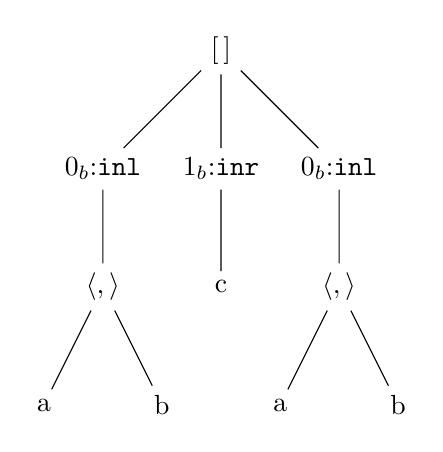
\begin{tikzpicture}[tlabel/.style={font=\footnotesize}]
\node{$[\,]$}
child{
node{$0_b$:\inl}
child{
node {$\langle,\rangle$}
child{node{a}}
child{node{b}}
}
}
child{
node{$1_b$:\inr}
child{node {c}}
}
child{
node{$0_b$:\inl}
child{
node {$\langle,\rangle$}
child{node{a}}
child{node{b}}
}
};
\end{tikzpicture}
\end{center}

\end{Example}


The relation between codes and its correspondent parse trees is specified in the next
theorem.

\begin{Theorem}
  Let $t$ be a parse tree such that $\vdash t : e$, for some RE e. Then $(\code\: t\: e) \rhd e$ and
  $\decodee\:(\code\: t\: e)\,: e = t$.
\end{Theorem}
\begin{proof}
  Induction on the derivation of $\vdash t : e$.
\end{proof}


\subsection{Dealing with problematic REs}\label{subsection:problematic}

A known problem in RE parsing is how to deal with the so-called problematic REs. A naive approach for 
parsing problematic REs can make the algorithm loop~\cite{Frisch2004}. Medeiros et al. \cite{Medeiros14}
present a function which converts a problematic RE into a equivalent non-problematic one.

The conversion function relies on two auxiliar definitions: one for testing if a RE accepts the empty string and 
another to test if a RE is equivalent to $\epsilon$. We name such functions as \nullable~ and \emptyy, 
respectively.

\[
\begin{array}{lcl}
   \nullable(\emptyset) & = & \bot \\ 
   \nullable(\epsilon)  & = & \top \\
   \nullable(a)         & = & \bot \\ 
   \nullable(e_1 + e_2) & = & \nullable(e_1)\lor\nullable(e_2)\\
   \nullable(e_1\:e_2)  & = & \nullable(e_1)\land\nullable(e_2)\\
   \nullable(e ^\star)  & = & \top \\
   \\
   \emptyy(\emptyset)    & = & \bot \\ 
   \emptyy(\epsilon)     & = & \top \\
   \emptyy(a)            & = & \bot \\
   \emptyy(e_1 + e_2)    & = & \emptyy(e_1) \land \emptyy(e_2)\\
   \emptyy(e_1\:e_2)     & = & \emptyy(e_1) \land \emptyy(e_2)\\
   \emptyy(e ^\star)     & = & \emptyy(e)\\        
\end{array}
\]

Functions \nullable~ and \emptyy~ obeys the following correctness properties.


\begin{Lemma}
   \nullable($e$) = $\top$ if, and only if, $\epsilon\in\sembrackets{e}$.
\end{Lemma}
\begin{proof}$\,$\\
  $(\to)$ Induction over the structure of $e$. \\$(\leftarrow)$ Induction over the derivation of $\epsilon \in\sembrackets{e}$.
\end{proof}

\begin{Lemma}
   If \emptyy($e$) = $\top$ then $e \approx \epsilon$.
\end{Lemma}
\begin{proof}
   Induction over the structure of $e$.
\end{proof}


Given these two predicates, Medeiros et.al.~\cite{Medeiros14} define two mutually recursive functions,
named \fin~ and \fout. The function \fout~ recurses over the structure of an input RE
searching for a problematic sub-expression and \fin~ rewrites the Kleene star subexpression
so that it becomes non-problematic and preserves the language of the original 
RE. The definition of functions \fin~ and \fout~ are presented next.

\[
\begin{array}{lcl}
   \fout(e) & = & e,\,\texttt{if } e = \epsilon, e = \emptyset \texttt{ or } e = a\\
   \fout(e_1 + e_2) & = & \fout(e_1) + \fout(e_2) \\
   \fout(e_1\:e_2) & = & \fout(e_1)\:\fout(e_2)\\
   \fout(e^\star) & = & \left\{
        \begin{array}{ll}
           \fout(e)^\star & \texttt{if } \neg\,\nullable(e)\\
           \epsilon       & \texttt{if } \emptyy(e)\\
           \fin(e)^\star  & \texttt{otherwise}
        \end{array}
                          \right.
\end{array}
\]

\[
\begin{array}{lcl}
   \fin(e_1\:e_2) & = & \fin(e_1+e_2)\\
   \fin(e_1 + e_2) & = & \left\{
             \begin{array}{ll}
                \fin(e_2)  & \texttt{if }\emptyy(e_1) \land \nullable(e_2)\\
                \fout(e_2) & \texttt{if }\emptyy(e_1) \land \neg \nullable(e_2)\\
                \fin(e_1)  & \texttt{if }\nullable(e_1) \land \emptyy(e_2)\\
                \fout(e_1) & \texttt{if }\neg \nullable(e_1) \land \emptyy(e_2)\\
                \fout(e_1) + \fin(e_2) & \texttt{if }\neg \nullable(e_1) \land \neg\emptyy(e_2)\\
                \fin(e_1) + \fout(e_2) & \texttt{if }\neg \emptyy(e_1) \land \neg \nullable(e_2)\\
                \fin(e_1) + \fin(e_2) & \texttt{otherwise}
             \end{array}
                         \right. \\
   \fin(e^\star) & = & \left\{
             \begin{array}{ll}
               \fin(e) & \texttt{if }\nullable(e)\\
               \fout(e) & \texttt{otherwise}\\
             \end{array}
                       \right.
\end{array}
\]

The result of applying \fout~ on a RE is producing an equivalent non-problematic one. This fact is expressed
by the following theorem. 

\begin{Theorem}
   If $\fout(e) = e'$ then $e \approx e'$ and $e'$ is a non-problematic RE.
\end{Theorem}
\begin{proof}
   Well-founded induction on the complexity of $(e,s)$, where $s$ is an arbitrary string, using
   several lemmas about RE equivalence and lemmas 1 and 2.
\end{proof}

This result is proved (informally\footnote{By ``informally'', we mean that the
  result is not mechanized in a proof assistant.}) by Medeiros et. al.~\cite{Medeiros14}. In order to formalize this result
in Coq, we needed to prove several theorems about RE equivalence. We postpone the discussion on some details
of our formalization to Section \ref{section:formalization}.


\section{Proposed semantics for RE parsing}\label{section:semantics}

In this section we present the definition of a big step operational semantics
for a RE parsing VM.
The state of our VM is a pair formed by the current RE and the string under parsing. Each machine 
transition may produce, as a side effect, a bit-coded parse tree and the remaining string to be 
parsed. We denote our semantics by a judgement of the form $\langle e, s \rangle \leadsto (bs,s_p,s_r)$,
where $e$ is current RE, $s$ is the input string, $bs$ is the produced bit-coded tree, $s_p$ is
the parsed prefix of the input string and $s_r$ is the yet to be parsed string.
We let notation $\langle e, s \rangle\not\leadsto$ denote the fact that string
$s$ cannot be parsed by RE $e$.

\begin{figure}[h]
  \[
     \begin{array}{ccc}
        \infer[_{\{EpsVM\}}]{\langle \epsilon, s\rangle \leadsto ([\,],\epsilon,s)}{} & &
        \infer[_{\{ChrVM\}}]{\langle a, as\rangle\leadsto ([\,],a,s)}{} \\ \\
        \infer[_{\{LeftVM\}}]{\langle e_1 + e_2,s\rangle\leadsto (0_b\,b,s_p,s_r)}{\langle e_1, s\rangle \leadsto (b,s_p,s_r)} & &
        \infer[_{\{RightVM\}}]{\langle e_1 + e_2,s\rangle\leadsto (1_b\,b,s_p,s_r)}{
                                                                \langle e_2, s\rangle \leadsto (b,s_p,s_r)} \\ \\
        \infer[_{\{CatVM\}}]{\langle e_1\:e_2,s\rangle\leadsto (b_1\,b_2,s_{p1}\,s_{p2},s_r)}
              {\begin{array}{c}
                  \langle e_1, s\rangle \leadsto (b_1,s_{p1},s_1) \\
                  \langle e_2, s_1\rangle \leadsto (b_2,s_{p2},s_r)
              \end{array}} & & 
        \infer[_{\{NilVM\}}]{\langle e^\star, s\rangle\leadsto
                               (1_b,\epsilon,s)}{\langle e, s \rangle
                               \not\leadsto}\\ \\

        \multicolumn{3}{c}{
           \infer[_{\{ConsVM\}}]{\langle e^\star, s\rangle\leadsto (0_b\,b_1\,b_2,s_{p1}\,s_{p2},s_r)}
                 {\langle e, s \rangle \leadsto (b_1,s_{p1},s_1) & s_{p1} \neq \epsilon &
                  \langle e^\star, s_1 \rangle \leadsto (b_2, s_{p2},s_r)}
        }
     \end{array}
  \]
  \caption{Operational semantics for RE parsing.}
  \label{figure:bigstepsemantics}
\end{figure}

The meaning of each semantics rules is as follows. Rule $EpsVM$ specifies that parsing $s$ using RE $\epsilon$ produces 
an empty list of bits and does not consume any symbol from $s$. Rule $ChrVM$ consumes the first symbol of the input string
if it matches the input RE.  Rules $LeftVM$ and 
$RightVM$ specifies how the semantics executes an RE $e + e'$, by trying to
parse the input using either the left or right subexpression. Note that, as a result, we append a bit $0_b$ when we successfully 
parse the input using the left choice operand and the bit $1_b$ for a parsing using the right operand. Rule $CatVM$ defines 
how a concatenation $e_1\,e_2$ is executed by the semantics: first, the input is parsed using the RE $e_1$ and the remaining 
string is used as input to execute $e_2$. The bit-coded tree for the $e_1\,e_2$ is just the concatenation of the produced 
codes for $e_1$ and $e_2$. Rules $NilVM$ and $ConsVM$ deal with unproblematic Kleene star REs. The rule $NilVM$ is only applicable when
it is not possible to parse the input using the RE $e$ in $e^\star$. Rule $ConsVM$ can be used whenever we can parse the
input using $e$ and the parsed prefix is not an empty string. The remaining string ($s_1$) of $e$'s parsing is used as
input for the next iteration of RE $e^\star$ parsing. 

Evidently, the proposed semantics is sound and complete w.r.t. standard RE
semantics and only produces valid parsing evidence.

\begin{Theorem}[Soundness]
  If $\langle e, s \rangle \leadsto (bs,s_p,s_r)$ then $s = s_p\,s_r$ and $s_p\in\sembrackets{e}$.
\end{Theorem}
\begin{proof}
  Well-founded induction on the complexity of $(e,s)$.
\end{proof}

\begin{Theorem}[Completeness]
  If $s_p\in\sembrackets{e}$ then for all $s_r$ we have that exists $bs$, s.t. $\langle e, s_p\,s_r \rangle \leadsto (bs,s_p,s_r)$.
\end{Theorem}
\begin{proof}
  Well-founded induction on the complexity of $(e,s)$.
\end{proof}

\begin{Theorem}[Parsing result soundness]
  If $\langle e, s \rangle \leadsto (bs,s_p,s_r)$ then: 1) $bs \rhd e$; 2) $\flatten(\decodee(bs : e)) = s_p$; and 3)
  $\code(\decodee(bs : e) : e) = bs$. 
\end{Theorem}
\begin{proof}
  Well-founded induction on the complexity of $(e,s)$ using Theorem 3.
\end{proof}

\section{Coq formalization}\label{section:formalization}

In this section we describe the main design decisions in our formalization. At
the end of this section, we discuss how we extract a Haskell implementation from
our Coq development
.

\paragraph{RE syntax and semantics} Our representation of RE syntax and
semantics is as usual in type theory-based proof assistants. We use an inductive
type to represent RE syntax and an inductive predicate to denote its semantics.

\begin{minted}{coq}
Inductive regex : Set :=
| Empty : regex | Eps : regex | Chr : ascii -> regex
| Cat : regex -> regex -> regex
| Choice : regex -> regex -> regex
| Star   : regex -> regex.
\end{minted}

Type \coq{regex} represents RE syntax and its definition is straightforward.
We use some notations to write \coq{regex} values. We let \verb|#0| denote
\coq{Empty}, \verb|#1| represents \coq{Eps}, while infix operators \coq{:+:} and
\coq{@} denote \coq{Choice} and \coq{Cat}. Finally, \coq{Star e} is
written \coq{(e ^*)}.

RE semantics is represented by type \coq{in_regex} which has a constructor for each
rule of the semantics presented in Figure~\ref{figure:resemantics}.

\begin{minted}{coq}
Inductive in_regex : string -> regex -> Prop :=
| InEps : "" <<- #1
| InChr : forall c, String c "" <<- ($ c)
| InLeft
  :  forall s e e'
  ,  s <<- e
  -> s <<- (e :+: e')
| InStarRight              
  : forall s s' e s1 
  , s <> ""  
  -> s <<- e
  -> s' <<- (e ^*)
  -> s1 = s ++ s'
  -> s1 <<- (e ^*)
...  (** some constructors omitted. *)
where "s '<<-' e" := (in_regex s e).
\end{minted}
We use notation \coq{s <<- e} to denote \coq{in_regex s e}.

\paragraph{RE equivalence} Using the previous presented semantics, we can define
RE equivalence by coding its standard definition in Coq as:
\begin{minted}{coq}
Definition regex_equiv (e e' : regex) : Prop :=
  forall s, s <<- e <-> s <<- e'.
\end{minted}
We use notation \coq{e1 === e2} to denote \coq{regex_equiv e1 e2}. In our
formalization, we proved that \coq{regex_equiv} is an equivalence relation,
which is necessary to allow the rewriting of such equalities by Coq
tactics.

In order to complete our formalization, we needed several results about RE
equivalence. Most of them are proved by well-founded induction on the complexity
of a pair formed by a RE and a string (defined in Section~\ref{subsection:resyntaxsemantics}).
In order to formalize the needed ordering relation, we take advantage of Coq's
standard library, which provide several combinators to assemble well-founded
relations. As an example, consider the following fact used by Medeiros et. al~\cite{Medeiros14} to
prove the correctness of its \fout~function: $(e_1 + e_2)^\star \approx
(e_1\,e_2)^\star$, which holds if both $e_1$ and $e_2$ accepts the empty string.
In our formalization such equivalence is proved by the following theorem proved
by well-founded induction.

\begin{minted}{coq}
Lemma choice_star_cat_star 
   : forall e1 e2, "" <<- e1 -> "" <<- e2 ->
                   ((e1 @ e2) ^*) === ((e1 :+: e2) ^*). 

\end{minted}
Several other lemmas about RE equivalence were proved in order to complete
the formalization of the problematic RE conversion function. We omit them
for brevity.

\paragraph{Converting problematic REs} The first step to certify the algorithm
for converting problematic REs into non-problematic ones is to define the
predicates for testing whether an input RE is nullable or whether it is equivalent to
$\epsilon$. We define such functions using dependently typed programming, i.e.
its types provide certificates that the result has its desired correctness
property.

The nullability test is represented by function \coq{null}:
\begin{minted}{coq}
Definition null : forall e, {"" <<- e} + {~ "" <<- e}.
  refine (fix null e : {"" <<- e} + {~ "" <<- e} :=
            match e as e' return e = e' -> 
                    {"" <<- e'} + {~ "" <<- e'} with
            | #1 => fun Heq => Yes
            | e1 @ e2 => fun Heq =>
               match null e1 , null e2 with
               | Yes , Yes  => Yes
               | _ , _   => No
               end 
            | e1 :+: e2 => fun Heq => ...
            | e1 ^* => fun Heq => Yes
            end (eq_refl e)) ...
          (** some cases and tactics omitted *)
\end{minted}
Its type specifies that for any RE $e$ either $e$ accepts the empty string (i.e.
\coq{"" <<- e} holds) or not (\coq{~ "" <<- e}). Since such function contains
proofs terms, we use tactic \coq{refine} to define its computation content
leaving the logical subterms to be filled by tactics. The definition of
\coq{null} employs the convoy-pattern~\cite{Chlipala13}, which consists in
introducing an equality to allow the refinement of each equation type in
dependently typed pattern-matching.

In order to specify the emptyness test predicate, we use an inductive type
which characterizes when a RE is equivalent to $\epsilon$.
\begin{minted}{coq}
Inductive empty_regex : regex -> Prop :=
| Emp_Eps : empty_regex #1
| Emp_Cat : forall e e', empty_regex e ->
                    empty_regex e' ->
                    empty_regex (e @ e')
| Emp_Choice : forall e e', empty_regex e ->
                    empty_regex e' ->
                    empty_regex (e :+: e')
| Emp_Star : forall e, empty_regex e ->
                  empty_regex (e ^*).
\end{minted}
The meaning of each constructor of \coq{empty_regex} is as follows:
\coq{Emp_Eps} specifies that the empty RE is equivalent to itself.
For concatenation, choice and Kleene star, we can only say that they are
equivalent to $\epsilon$ if all of its subterms are also equivalent
to the empty RE.

Using the \coq{empty_regex} predicate we can easily prove the following
theorems. The first specifies that if \coq{empty_regex e} holds then
\coq{e} accepts the empty string and the second says that if
\coq{empty_regex e} is provable then \coq{e} is equivalent to the empty
string RE.

\begin{minted}{coq}
Lemma empty_regex_sem : forall e, empty_regex e -> "" <<- e.
Theorem empty_regex_spec : forall e, empty_regex e -> e === #1.
\end{minted}

The emptiness test function follows the same definition pattern as \coq{null}
using the \coq{refine} tactic. We specify its type using \coq{empty_regex}
predicate and we omit its definition for brevity.

Having defined these two predicates, we can implement the function to
convert problematic REs into non-problematic ones. The specification
of when a RE is not problematic is given by the following inductive predicate. 
\begin{minted}{coq}
Inductive unproblematic : regex -> Prop :=
| UEmpty : unproblematic #0
| UEps   : unproblematic #1
| UChr   : forall c, unproblematic ($ c)
| UCat   : forall e e', unproblematic e ->
                   unproblematic e' ->
                   unproblematic (e @ e')
| UChoice : forall e e', unproblematic e ->
                    unproblematic e' ->
                    unproblematic (e :+: e')
| UStar : forall e, ~ ("" <<- e) -> 
                   unproblematic e -> 
                   unproblematic (Star e).
\end{minted}
Type \coq{unproblematic} says that empty set, empty string and single
characters REs are unproblematic. Concatenation and choice REs are
unproblematic if both its subexpression are unproblematic. Finally,
a Kleene star is unproblematic if its subexpression is unproblematic and
does not accept the empty string. Finally, we specify the problematic RE
conversion function with the following type:
\begin{minted}{coq}
Definition unprob 
   : forall (e : regex), {e' | e === e' /\ unproblematic e'}.
\end{minted}
Function \coq{unprob} type says that from a input RE \coq{e} it returns another
RE \coq{e'} which is unproblematic and equivalent to \coq{e}. Again, we define
\coq{unprob} using \coq{refine} tactic and its definition is just the
Coq coding of \fout. As pointed by Medeiros et. al.~\cite{Medeiros14}, most of
the work to produce a unproblematic RE is done by function \fin, which is
applied when the inner RE of a Kleene star accepts the empty string and is not
equivalent to the empty RE. Function \coq{unprob_rec} implements \fin function
and we specify it with the following type:
\begin{minted}{coq}
Definition unprob_rec : forall e, "" <<- e -> ~ empty_regex e -> 
    {e' | (e ^*) === (e' ^*) /\ ~ "" <<- e' /\ unproblematic e'}
\end{minted}
\coq{unprob_rec}'s type estabilishes that the return RE \coq{e'} is unproblematic, does not
accepts the empty string and that its Kleene star is equivalent to input REs
Kleene star, i.e.  \coq{(e ^*) === (e' ^*)}.

\paragraph{Parse trees and bit-code representation}

In our formalization, we use the following inductive type to represent parse
trees:

\begin{minted}{coq}
Inductive tree : Set :=
| TUnit  : tree | TChr   : ascii -> tree
| TCat   : tree -> tree -> tree 
| TLeft  : tree -> tree | TRight : tree -> tree 
| TNil   : tree | TCons  : tree -> tree -> tree.
\end{minted}

Constructor \coq{TUnit} denotes a parse tree for the empty string RE,
\coq{TChr} the tree for a single symbol RE and \coq{TCat} the tree for
the concatenation of two REs. \coq{TLeft} and \coq{TRight} denote trees
for the choice operator. Constructors \coq{TCons} and \coq{TNil} can be
used to form a list of trees for a Kleene star RE.

The parse tree typing judgement is
coded as the following inductive predicate, in which each constructor
has a correspondent rule in Figure~\ref{figure:parsetreetyping}.

\begin{minted}{coq}
Inductive is_tree_of : tree -> regex -> Prop :=
| ITUnit : TUnit :> #1
| ITChr  : forall c, (TChr c) :> ($ c)
| ITCat  : forall e t e' t',
    t :> e   ->
    t' :> e' ->
    (TCat t t') :> (e @ e')
| ITLeft : forall e t e',
    t :> e ->
    (TLeft t) :> (e :+: e')
| ITRight : forall e e' t',
    t' :> e' ->
    (TRight t') :> (e :+: e')
| ITNil : forall e, TNil :> (Star e)
| ITCons : forall e t ts,
    t :> e ->
    ts :> (Star e) ->
    (TCons t ts) :> (Star e)
where "t ':>' e" := (is_tree_of t e).
\end{minted}
Function \flatten~has a direct encoding as a Coq recursive definition and
we omit it for brevity. From \flatten~ and tree typing relation definitions,
theorems \ref{theorem:semanticstypingflatten} and
\ref{theorem:typingflattensemantics} are easily proved.

Bit coding of parse trees is represented by a list of bits, as follows:
\begin{minted}{coq}
Inductive bit : Set := O : bit | I : bit.
Definition code := list bit.
\end{minted}
The typing relation for bit-coded parse trees
(Figure~\ref{figure:typing-bitcodes}) has an immediate definition as an
inductively defined Coq relation.
\begin{minted}{coq}
Inductive is_code_of : code -> regex -> Prop :=
| ICEpsilon : [] :# #1
| ICChar    : forall c, [] :# ($ c)
| ICLeft    : forall bs e e'
  , bs :# e ->
    (O :: bs) :# (e :+: e')
| ICRight   : forall bs e e'
  , bs :# e' ->
    (I :: bs) :# (e :+: e')
| ICCat : forall bs bs' e e'
  , bs :# e ->
    bs' :# e' ->
    (bs ++ bs') :# (e @ e')
| ICNil : forall e, (I :: []) :# (e ^*)
| ICCons : forall e bs bss, 
    bs :# e -> 
    bss :# (e ^*) -> 
    (O :: bs ++ bss) :# (e ^*) 
where "bs ':#' e" := (is_code_of bs e).
\end{minted}
As with \flatten, function \code~ has an immediate Coq definition. The next
results about \code~are proved by a routine inductive proof.
\begin{minted}{coq}
Lemma encode_sound
  : forall bs e, bs :# e -> exists t, t :> e /\ encode t = bs.
Lemma encode_complete
  : forall t e, t :> e -> (encode t) :# e.   
\end{minted}
Unlike \code, function \decodee~ has a more elaborate recursive definition, as
shown in Section~\ref{subsection:bitcodedparsetrees}, since it recurses over the
input RE while threading the remaining bits to be parsed into a tree. Since it
has a more complicated definition, we use dependent types to combine its definition
with its correctness proof. First, we define type \coq{nocode_for} which
denotes proofs that some bit list is not a valid bit-coded tree for some RE.
\begin{minted}{coq}
Inductive nocode_for : code -> regex -> Prop :=
| NCEmpty : forall bs, nocode_for bs #0
| NCChoicenil : forall e e', nocode_for [] (e :+: e')
| NCLBase : forall bs e e', 
    nocode_for bs e -> 
    nocode_for (O :: bs) (e :+: e')
| NCRBase : forall bs e e', 
    nocode_for bs e' -> 
    nocode_for (I :: bs) (e :+: e')
| NCStarnil : forall e, nocode_for [] (e ^*)
| NCStar : forall bs bs1 bs2 e,
      is_code_of bs1 e ->
      nocode_for bs2 (e ^*) ->
      bs = O :: bs1 ++ bs2  ->
      nocode_for bs (e ^*)
| NCStar1 : forall bs e,
    nocode_for bs e ->
    nocode_for (O :: bs) (e ^*).
(** some code omitted *)
\end{minted}
Constructor \coq{NCEmpty} specifies that there is no code for the empty set RE,
\coq{#0}. For choice REs, we have several cases to cover. Constructor
\coq{NCChoicenil} specifies that the empty list is not a valid code for any
choice RE. Constructor \coq{NCLBase} (\coq{NCRBase}) specifies that if a list
isn't a valid code for a RE \coq{e} (\coq{e'}) it cannot be used to form a valid
code for \coq{e :+: e'}. In order to build a proof that some bit list isn't a
valid code for a concatenation RE, we just need to prove that it is not a code
for some of its sub-expressions. Finally, for the Kleene star, we have some
cases to cover: first, constructor \coq{NCStarnil} shows that the empty list
cannot be a code for any star RE. For non-empty bit-lists, it is just necessary
to show that some part of the bit list isn't a code either for \coq{e} or
\coq{e ^*}.

Using predicate \coq{nocode_for} we can define a type for invalid bit-codes:
\begin{minted}{coq}
Definition invalid_code bs e :=
  nocode_for bs e \/ exists t b1 bs1, bs = (code t) ++ (b1 :: bs1).
\end{minted}
which basically says that a bit list is an invalid code for a RE \coq{e} when
either we can construct a proof of \coq{nocode_for} or we can parse a prefix of it into a
valid tree but it leaves a non-empty bit list as a remaining suffix. Using this
infrastructure, we can define the decode function with the following type:
\begin{minted}{coq}
Definition decode e bs : 
   {t | bs = code t /\ is_tree_of t e} + {invalid_code bs e}.
\end{minted}
Note that the previous type denotes the correctness property of a decode
function: either it returns a valid tree for the input RE that can be
converted into the input bit list or a proof that such bit list isn't a valid
code for the input RE.

\paragraph{Formalizing the proposed semantics and its interpreter}

Our semantics definition consists of the Coq representation of the judgement in
Figure~\ref{figure:bigstepsemantics}, which is presented below.
\begin{minted}{coq}
Inductive in_regex_p : string -> regex -> 
                       string -> string -> Prop :=
| InEpsP
  : forall s, s <$- #1 ; "" ; s
| InChrP
  : forall a s,
    (String a s) <$- ($ a) ; (String a "") ; s
| InLeftP
  : forall s s' e e',
    (s ++ s') <$- e ; s ; s' ->
    (s ++ s') <$- (e :+: e') ; s ; s'
| InCatP : forall s s' s'' e e',
    (s ++ s' ++ s'') <$- e ; s ; (s' ++ s'') ->
    (s' ++ s'') <$- e' ; s' ; s'' ->
    (s ++ s' ++ s'') <$- (e @ e') ; (s ++ s') ; s''
| InStarRightP : forall s1 s2 s3 e,
    s1 <> "" ->
    (s1 ++ s2 ++ s3) <$- e ; s1 ; (s2 ++ s3) ->
    (s2 ++ s3) <$- (Star e) ; s2 ; s3 ->
    (s1 ++ s2 ++ s3) <$- (Star e) ; (s1 ++ s2) ; s3
where "s '<$-' e ';' s1 ';' s2" := (in_regex_p s e s1 s2).
(** some code omitted *)
\end{minted}
In order to ease the task of writing types involving \coq{in_regex_p}, we define
the following notation \coq{s <$- e ; s1 ; s2$} for \coq{in_regex_p s e s1 s2}.
The meaning of \coq{in_regex_p} is the same as the rules of our semantics
in Figure~\ref{figure:bigstepsemantics} and we omit redundant explanations for
brevity.

The soundness and completeness theorems of the proposed semantics are stated below.
Both are proved by induction on the complexity of the pair $(e,s)$.
\begin{minted}{coq}
Theorem in_regex_p_complete : 
   forall e s, s <<- e -> forall s', (s ++ s') <$- e ; s ; s'.
Theorem in_regex_p_sound : 
   forall e s s1 s', s <$- e ; s1 ; s' -> 
                     s = s1 ++ s' /\ s1 <<- e.
\end{minted}
The completeness express that if an string \coq{s} is in the language of RE
\coq{e}, i.e. \coq{s <<- e}, then our semantics can parse the string \coq{s ++
  s'}, for any string \coq{s'}. Soundness theorem says that whenever we have
a derivation \coq{s <$- e ; s1 ; s'}, then we have that the input string
\coq{s} should be equal to the concatenation of the parsed prefix (\coq{s1}) and
the remainder (\coq{s'}), i.e. \coq{s = s1 ++ s'}, and the parsed prefix should
be in \coq{e}'s language (\coq{s1 <<- e}).

After a proper definition of our semantics, we developed a formalized
interpreter for it. First, we need to define a type to store the
intermediate results of the VM. We call this type \coq{result} and its
definition is shown below.
\begin{minted}{coq}
Record result : Set
  := Result {
      bitcode   : code
    ; consumed  : string  
    ; remaining : string
    }.
\end{minted} 
Type \coq{result} has a obvious meaning: it stores the computed bit-coded parse
tree, the consumed prefix of the input string and its remaining suffix. Using
type \coq{result}, we can define the specification of our interpreter as:
\begin{minted}{coq}
Definition interp  : forall e s,
 {{r | exists e', unproblematic e' /\ e === e'  /\
   s = consumed r ++ remaining r /\
   (consumed r ++ remaining r) <$- e' ; consumed r ; remaining r /\
   (bitcode r) :# e'}}. 
\end{minted}
Function \coq{interp} is defined as follows: first it converts the input RE into
an equivalent unproblematic one and then proceed to parse the input string by
well-founded recursion on the complexity of the pair $(e,s)$. In its definition,
we follow the same pattern used before: the computational content is specified
using tactic \coq{refine} to mark proof positions using holes that are filled
later by tactics.

\paragraph{Extracting a certified implementation}

In order to obtain a certified Haskell implementation from our VM-based algorithm,
we use Coq support for extraction, which has several pre-defined
settings for using data-types and functions of Haskell's
Prelude\footnote{Prelude is the name of the Haskell library automatically loaded
in any Haskell module~\cite{Haskell98}.}.

The extracted Haskell code for our VM interpreter has 259 lines. In order to use 
the algorithm, we build a grep-like command line tool, which is avaliable at 
project's on-line repository~\cite{regexvm-rep}. 

\section{Experimental results}\label{section:experiments}

We use the formalized algorithm to build a Haskell tool for RE parsing and
compare its performance against the library
regex-applicative~\cite{regex-applicative}, which is an optimized library for RE
matching / parsing for Haskell. The reason for choosing this library is that it allows us to 
build bit coded parse trees using its applicative interface~\cite{Mcbride2008},
enabling a more fair comparison with our algorithm.
We ran our experiments on a machine with a Intel Core I7 1.7 GHz, 8GB RAM 
running Mac OS X 10.14.2; the results were collected and the average of several 
test runs were computed. In order to allow reproducibility, the on-line
repository contains a Haskell program that automates the task of running the 
experiments to produce the graphs presented next.

Also, we would like to emphasize that the intent of these experiments is not to
conclude that the proposed algorithm is more (less) efficient than the chosen 
library for RE parsing. Our main objective is to show that a fully verified
algorithm can have a performance comparable to an optimized library to the 
same task. 

The first experiment consists in parsing strings formed by a's by RE 
$(a + b + ab)^\star$ and the second with strings formed by ab's 
(examples taken from~\cite{Sulzmann14}). The results are presented in Figures
~\ref{fig:graph1} and~\ref{fig:graph2}.

\begin{figure}[h]
  \centering
  \begin{minipage}{0.45\textwidth}
    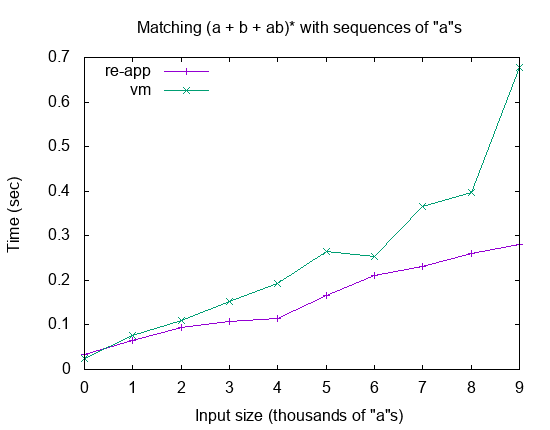
\includegraphics[width=.9\textwidth]{as.png}
    \caption{Results of experiment 1.}
    \label{fig:graph1}
  \end{minipage} \hfill
  \begin{minipage}{0.45\textwidth}
    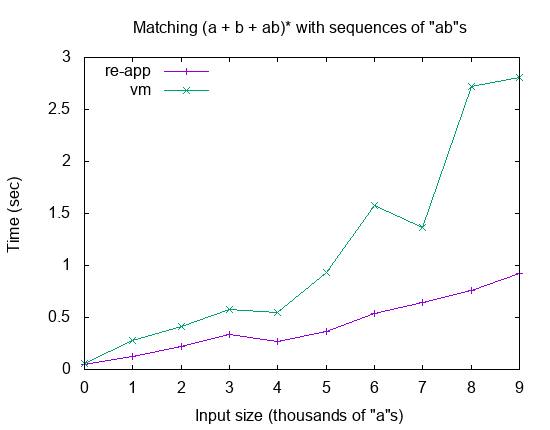
\includegraphics[width=.9\textwidth]{abs.png}
    \caption{Results of experiment 2.}
    \label{fig:graph2}
  \end{minipage}
\end{figure}

When compared with regex-applicative, our tool exhibits a bad performance in
this test (around 2 to 3 times slower than regex-applicative). The main reason for 
such behaviour can be explained by the implementation details of
regex-applicative,  which internally compiles a RE 
to a NFA to parse the input string. Since the RE used in this test is short,
converting it into a NFA does not influence in the library execution time.


Another experiment considered was to parse strings $a^n$ by the RE $(a +
\epsilon)^na^n$, where $a^n$ denotes $n \geq 0$ copies of $a$. Such RE pose a 
chalenge to RE parsing algorithms since they need to simulate the traversal of
$2^n$ paths, by backtracking, before finding a match~\cite{Lasse2011}. The
results of executing this experiments on increasing values of $n$ is presented 
below.


\begin{figure}[h]
  \centering
  \begin{minipage}{0.45\textwidth}
    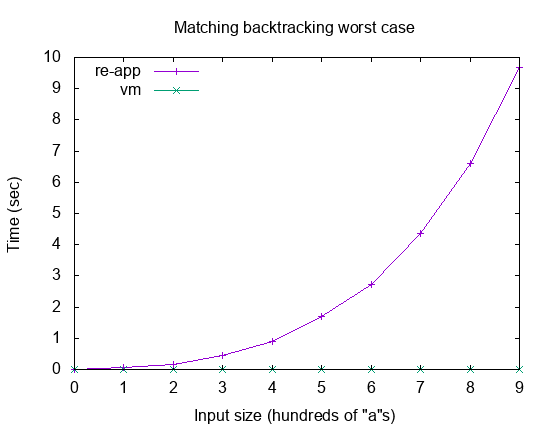
\includegraphics[width=.9\textwidth]{backtrack.png}
    \caption{Results of experiment 3.}
    \label{fig:graph3}
  \end{minipage} \hfill
  \begin{minipage}{0.45\textwidth}
    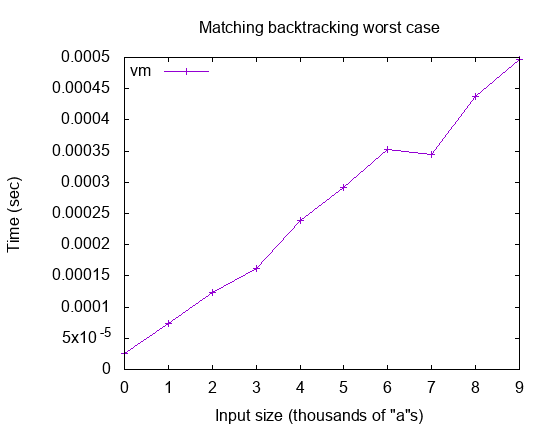
\includegraphics[width=.9\textwidth]{backtrack1.png}
    \caption{Results of experiment 3 considering only the VM.}
    \label{fig:graph4}
  \end{minipage}
\end{figure}

In this example, our approach has a much better performance than
regex-applicative, which exhibits an exponential behaviour (also known as
catastrophic backtracking~\cite{Kirrage13}). Such bad 
behaviour on large REs can be explained by the NFA-based parsing algorithm  
used by regex-applicative library. Notice that our VM-based algorithm shows 
a linear performance on such problematic inputs, as presented in
Figure~\ref{fig:graph4}.

The last experiment considered is to test how both approaches perform
on random generated REs and random accepted strings for them. In order to
perform such test, we use Haskell library QuickCheck~\cite{Claessen2000}.
The experiment consists in collecting the result of running both semantics 
on thousands of input pairs formed by a RE and strings. The average of such 
executions is presented in the Figure~\ref{fig:graph5}, which shows that both 
algorithms exhibit a linear behaviour  on random inputs.

\begin{figure}[h]
    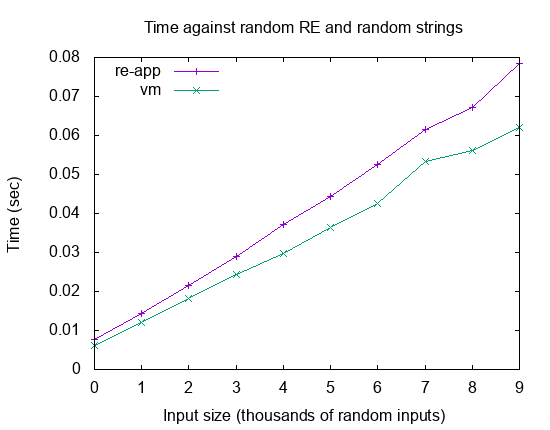
\includegraphics[width=0.6\textwidth]{random.png}
   \centering
   \caption{Results of experiment 4.}
   \label{fig:graph5}
\end{figure}

A few words should be written about how we generate random inputs
\footnote{We
  assume that the reader has some acquaintance with Haskell programming language
and its library for property based testing, QuickCheck. Good introductions to
Haskell are avaliable elsewhere~\cite{Lipovaca2011}.}. 
Generation of random RE is done by function \haskell{sizedRegex} with takes a depth limit to restrict
the size of the generated RE. Whenever the input depth limit is less or equal to 1, we can
only build a $\epsilon$ or a single character RE. The definition of \haskell{sizedRegex} uses
QuickCheck function \haskell{frequency}, which receives a list of pairs formed by a weight and
a random generator and produces, as result, a generator which uses such frequency distribution.
In \haskell{sizedRegex} implementation we give a higher weight to generate characters and equal distributions
to build concatenation, union or star.

\begin{minted}{haskell}
sizedRegex :: Int -> Gen Regex
sizedRegex n
  | n <= 1 = frequency [ (10, return Eps), (90, Chr <$> genChar) ]
  | otherwise = frequency [ (10, return Epsilon), (30, Chr <$> genChar)
         , (20, Cat <$> sizedRegex n2 <*> sizedRegex n2)
         , (20, Choice <$> sizedRegex n2 <*> sizedRegex n2)
         , (20, Star  <$> sizedRegex n2)]
         where n2 = div n 2
\end{minted}


Given an RE $e$, we can generate a random string $s$ such that $s \in\sembrackets{e}$
using the next definition. We generate strings by choosing randomly between branches of
a union or by repeating $n$ times a string $s$ which is accepted by $e$, whenever we
have $e^\star$ (function \haskell{randomMatches}).

\begin{minted}{haskell}
randomMatch :: Regex -> Gen String
randomMatch Eps = return ""
randomMatch (Chr c) = return [c]
randomMatch (Cat e e') = liftM2 (++) (randomMatch e)
                                     (randomMatch e')
randomMatch (Choice e e') = oneof [ randomMatch e, randomMatch e' ]
randomMatch (Star e) = do
      n <- choose (0,3) :: Gen Int
      randomMatches n e

randomMatches :: Int -> Regex -> Gen String
randomMatches m e'
  | m <= 0 = return []
  | otherwise = liftM2 (++) (randomMatch e')
                            (randomMatches (m - 1) e')
\end{minted}

\section{Related works}\label{section:related}

Ierusalimschy~\cite{Ierusalimschy2009} proposed the use of Parsing Expression Grammars (PEGs) as a basis
for pattern matching. He argued that pure REs are a weak formalism for pattern-matching tasks:
many interesting patterns either are difficult to to describe or cannot be described by REs. He also said
that the inherent non-determinism of REs does not fit the need to capture specific parts of a match. Following
this proposal, he presented LPEG, a pattern-matching tool based on PEGs for the Lua language. He
argued that LPEG unifies the ease of use of pattern-matching tools with the full expressive power of PEGs.
He also presented a parsing machine that allows an implementation of PEGs for pattern matching.
Medeiros et. al.~\cite{Medeiros2008} presents informal correctness proofs of LPEG parsing machine.
While such proofs represent an important step towards the correctness of LPEG, there is no guarantee that LPEG
implementation follows its specification.

Rathnayake and Thielecke~\cite{Rathnayake2011} formalized a VM implementation for RE matching using
operational semantics. Specifically, they derived a series of abstract machines, moving from the abstract
definition of matching to realistic machines. First, a continuation is added to the operational semantics
to describe what remains to be matched after the current expression. Next, they represented the expression
as a data structure using pointers, which enables redundant searches to be eliminated via testing for pointer
equality. Although their work has some similarities with ours (a VM-based parsing of REs), they did not present
any evidence or proofs that their VM is correct.

Fischer, Huch and Wilke~\cite{Fischer2010} developed a Haskell program for matching REs. Their program is purely
functional and it is overloaded over arbitrary semirings, which solves the matching problem and supports other
applications like computing leftmost longest matchings or the number of matchings. Their program can also be used
for parsing every context-free language by taking advantage of laziness. Their developed program is based on an
old technique to turn REs into finite automata, which makes it efficient compared to other similar approaches.
One advantage of their implementation over our proposal is that their approach works with context-free languages,
not only with REs purely. However, they did not present any correctness proof of their Haskell code.

Cox~\cite{Cox2009} said that viewing RE matching as executing a special machine makes it possible to add new
features just by the inclusion of new machine instructions. He presented two different ways to implement
a VM that executes a RE that has been compiled into  byte-codes: a recursive and a non-recursive
backtracking implementation, both in C programming language. Cox's work on VM-based RE parsing is poorly specified:
both the VM semantics and the RE compilation process are described only informally
and no correctness guarantees are even mentioned.

Frisch and Cardelli~\cite{Frisch2004} studied the theoretical problem of matching a flat sequence against a type (RE): the
result of the process is a structured value of a given type. Their contributions were in noticing that: (1) A disambiguated
result of parsing can be presented as a data structure that does not contain ambiguities. (2) There are problematic cases in
parsing values of star types that need to be disambiguated. (3) The disambiguation strategy used in XDuce and CDuce (two
XML-oriented functional languages) pattern matching can be characterized mathematically by what they call greedy RE matching.
(4) There is a linear time algorithm for the greedy matching. Their approach is different since they want to axiomatize abstractly
the disambiguation policy, without providing an explicit matching algorithm. They identified three notions of problematic words, REs,
and values (which represent the ways to match words), related these three notions, and proposed matching algorithms to deal with the
problematic case.

Ribeiro and Du Bois~\cite{Ribeiro2017} described the formalization of a RE parsing algorithm that produces a bit representation
of its parse tree in the dependently typed language Agda. The algorithm computes bit-codes using Brzozowski derivatives and
they proved that the produced codes are equivalent to parse trees ensuring soundness and completeness with respect to an
inductive RE semantics. They included the certified algorithm in a tool developed by themselves, named verigrep, for RE-based
search in the style of GNU grep. While the authors provided formal proofs, their tool show a bad performance when compared to
other approaches to RE parsing.

Nielsen and Henglein~\cite{Lasse2011} showed how to generate a compact bit-coded representation of a parse tree for a
given RE efficiently, without explicitly constructing the parse tree first, by simplifying the DFA-based parsing algorithm of
Dubé and Feeley~\cite{Dube2000} to emit a bit representation without explicitly materializing the parse tree itself.
They also showed that Frisch and Cardelli’s greedy RE parsing algorithm~\cite{Frisch2004} can be straightforwardly modified to
produce bit codings directly. They implemented both solutions as well as a backtracking parser and performed benchmark experiments
to measure their performance. They argued that bit codings are interesting in their own right since they are typically not
only smaller than the parse tree, but also smaller than the string being parsed and can be combined with other techniques for
improved text compression. As others related works, the authors did not present a formal verification of their implementations.

Sulzmann et. al.~\cite{Sulzmann14} propose an algorithm for POSIX RE parsing
with uses RE derivatives to construct parse trees incrementally to solve both 
matching and submatching for REs. In order to improve the
efficiency of the proposed algorithm, Sulzmann et al. use a bit encoded representation of RE parse trees. Textual proofs of
correctness of the proposed algorithm are presented in an appendix.
Ausaf et. al.~\cite{Ausaf16} present a Isabelle/HOL formalization of Sulzmann et. al POSIX
parsing algorithm. They gave their inductive definition of what a
POSIX value is and showed that such a value is unique for a given RE and a
string being matched. We intend, as future work, to use a similar inductive
definition to characterize the disambiguation strategy followed by our VM semantics.

A recent application of REs was presented by Radanne \cite{Radanne2019}. In many
cases, the goal of a RE is not only to match a given text, but also to extract 
information from it. With that in mind, the author presented a technique to 
provide type-safe extraction based on the typed interpretation of REs. That 
technique relies on two-layer REs in which the upper layer allows to compose and 
transform data in a well-typed way, while the lower one is composed by untyped
REs that can leverage features from a preexisting RE matching engine. Results 
showed that this technique is faster than other two libraries that perform the 
same task, despite its lack of efficiency when compared with some full RE 
parsing algorithms. No formalization was provided in that work.

Radanne and Thiemann \cite{radanne:hal-01788827} pointed that some of the
algorithms for RE matching are rather intricate and the natural question 
that arises is how to test these algorithms. It is not too hard to come 
up with generators for strings that match a given RE, but on the other hand, 
the algorithms should reject strings that do not match that RE. So it is 
equally important to come up with strings that do not match. In other words, 
a satisfactory solution for testing such matchers would require generating 
positive as well as negative examples for some language. Thus, the authors 
presented an algorithm to generate the language of a generalized RE with union, 
intersection and complement operators. Using this technique, they could generate 
both positive and negative instance of a RE. They provided two implementations: 
one in Haskell, which explores different algorithmic improvements, and one in 
OCaml, which evaluates choices in data structures. Their algorithm lacks of 
correctness proofs. 

Groz and Maneth \cite{Groz2017} approached the efficiency of testing and
matching of deterministic REs. They presented a linear time algorithm for
testing whether a RE is deterministic and an efficient algorithm for matching
 words against deterministic REs. It was shown that an input word of length 
$n$ can be matched against a deterministic RE of length $m$ in time 
$O (m + n  \log \log m)$. If the deterministic RE has bounded depth 
of alternating union and concatenation operators, then matching can be
 performed in time $O (m + n)$. According to the authors, these results 
extend to REs containing numerical occurrence indicators. The authors 
presented the concept of deterministic REs and the differences between weak 
and strong determinism. Their paper contains some proofs, many of them related 
to algorithmic running time. However, their approach was focused on performance 
over deterministic REs, leaving aside the non-deterministic ones. We intend to 
investigate time complexity of algorithm in future works. 

A formal constructive theory of RLs was presented by Doczkal et. al. in
\cite{Doczkal2013}. They formalized some fundamental results about RLs. 
For their formalization, they used the Ssreflect extension to Coq, which 
features an extensive library with support for reasoning about finite 
structures such as finite types and finite graphs. They established all 
of their results in about 1400 lines of Coq, half of which are specifications. 
Most of their formalization deals with translations between different 
representations of RLs, including REs, DFAs, minimal DFAs and NFAs. 
They formalized all these (and other) representations and constructed 
computable conversions between them. Besides other interesting aspects 
of their work, they proved the decidability of language equivalence 
for all representations. Unlike our work, Doczkal et. al.'s only concerns 
about formalizing classical results of RL theory in Coq, without using the 
formalized automata in practical applications, like matching or parsing.  

A new technique for constructing a finite deterministic automaton from a 
RE was presented by Asperti et al in \cite{Asperti10}. It's based on the 
idea of marking a suitable set of positions inside the RE, intuitively 
representing the possible points reached after the processing of an initial 
prefix of the input string. In other words, the points mark the positions 
inside the RE which have been reached after reading some prefix of the 
input string, or better positions where the processing of the remaining 
string has to be started. Each pointed expression for a RE $e$ represents 
a state of the deterministic automaton associated with $e$; since there 
is obviously only a finite number of possible labellings, the number 
of states of the automaton is finite. The authors argued that 
Pointed REs join the elegance and the symbolic appealingsness of 
Brzozowski's derivatives with the effectiveness of McNaughton and 
Yamada's labelling technique, essentially combining the best of the 
two approaches, allowing a direct, intuitive and easily verifiable 
construction of the deterministic automaton for $e$. The authors said 
that pointed expressions can provide a more compact description for 
RLs than traditional REs. However, the authors do not discuss the 
usage of pointed REs for parsing or matching.

The concept of prioritized transducers to formalize capturing groups in RE
matching was introduced by Berglund and Merwe \cite{Berglund2016}. Their main
goal was to provide an automata-based theoretical foundation for the basic
functionality of modern RE matchers (with a focus on the Java RE standard
library). Many RE matching libraries perform matching as a form of parsing by 
using capturing groups, and thus output what subexpression matched which
substring. Their approach permits an analysis of matching semantics of a 
subset of the REs supported in Java. According to the authors, converting REs 
to what they called as prioritized transducers is a natural generalization of 
the Thompson construction for REs to NFA.

\section{Conclusion}\label{section:conclusion}

In this work, we presented a big-step operational semantics for a virtual machine for RE parsing. 
Our semantics produces, as parsing evidence, bit-codes which can be used to characterize which
disambiguation strategy is followed by the semantics. In order to avoid the well-known problems with 
problematic REs, we use an algorithm that converts a problematic RE into an equivalent non-problematic one.
All theoretical results reported in this paper are intregrally verified using
Coq proof assistant. 
From our formalization, we extract a Haskell implementation of our algorithm and used it to build 
a tool for RE parsing, which has performance comparable to a optimized Haskell library
for RE parsing. The complete development is avaliable at~\cite{regexvm-rep}.

As future work we intend to extend our semantics with some real-world regex
features like capture groups and quantifiers, while keeping an easy to follow
formalization and an efficient algorithmic interpreter for it. Other line of
research we intend to pursue is to formalize that the proposed semantics follow 
a disambiguation strategy and to investigate the time complexity of our
algorithm.

\section*{Acknowledgements}

This work is supported by the CNPq – Brazil under grant No.: 426232/2016.

\section*{References}

\bibliography{references}

\end{document}
